%------------------------------------------------------------------------------
% Define title, author(s), affiliation and publishing status
%
\papertitle%[Succesfully testing an on-board Superlaser System] % Short title used in healines (optional)
{%
 Domain validation for flow around a wing section% THE COMMENT SYMBOL AT THE END OF THIS LINE IS NEEDED
}%
%
\papertoctitle{Domain validation for flow around a wing section} % Title for toc
%
\paperauthor[Negi \etal] % Short authors used in headlines and List Of Papers
{%
  P. S. Negi, R. Vinuesa % D. S. Henningson and P. Schlatter%
}%
%
\listpaperauthor{Negi, Vinuesa}%, Henningson \& Schlatter}% (optional) Short authors used in List Of Papers
%
\paperaffiliation
{%
%  $^1$ Linn\'e FLOW Centre, KTH Mechanics, S-100 44 Stockholm, Sweden\\%
%  $^2$ Super-laser LAB, The Death Star, not orbiting Alderaan anymore ;)%
  Linn\'e FLOW Centre, KTH Mechanics, S-100 44 Stockholm, Sweden\\
  Swedish e-Science Research Centre (SeRC), SE-100 44, Stockholm, Sweden%
}%
%
\paperjournal[J. Num. Force] % Short publish info used in List Of Papers
{%
	Journal of the Numerical Force%
}%
%
\papervolume{51}%
%
%\papernumber{1}
%
\paperpages{123--122}%
%
\paperyear{3640}%
%
\papersummary%
{% Insert summary of the paper here (used in introduction) 
	A domain validation study is performed for large-eddy simulation of flow around a wing section at a chord-based Reynolds number of $Re_{c}=100,000$ in order to determine an optimum domain size. In a C-grid mesh topology, this optimum is found such that the far-field boundaries are 2 chords away from the airfoil and the outflow boundary is 3 chords downstream of the trailing edge.
}%
%
\graphicspath{{validation/imgs/}}%
%
%
%===============================================================================
%                            BEGIN PAPER
%===============================================================================
%
\begin{paper}

\makepapertitle

%------------------------------------------------------------------------------
% Abstract
%------------------------------------------------------------------------------
%
\begin{paperabstract}
	A domain validation study is performed for large-eddy simulation of flow around a wing section at a chord-based Reynolds number of $Re_{c}=100,000$ in order to determine an optimum domain size. It is found that keeping the far-field boundaries at 2 chord lengths from the airfoil and the outflow boundary at 3 chords downstream of the trailing edge, flow distortion is minimized and further increase in the domain size causes negligible changes in the mean flow and Reynolds stresses. 
        \keywords{wing, les}
\end{paperabstract}


%------------------------------------------------------------------------------
% Article
%------------------------------------------------------------------------------
%
%\documentclass[12pt, twocolumn]{article}
%\usepackage{helvet}
%
%\usepackage{epsfig}
%\usepackage[latin1]{inputenc}
%\begin{document}
%
%\title{Emulating Von Neumann Machines and Massive Multiplayer Online Role-
%Playing Games}
%\author{Mickey Mouse, Goofy G. Goof and Donald Duck}
%
%\date{}

%\maketitle




%\section*{Abstract}
%
% Many computational biologists would agree that, had it not been for
% Byzantine fault tolerance, the synthesis of replication that made
% developing and possibly investigating erasure coding a reality might
% never have occurred. In this work, we prove  the synthesis of linked
% lists. Even though such a hypothesis at first glance seems
% counterintuitive, it always conflicts with the need to provide
% object-oriented languages to systems engineers. APER, our new framework
% for mobile archetypes, is the solution to all of these grand
% challenges.

\section{Introduction}

Wind/water tunnels as well as numerical simulations serve as helpful tools for the investigation of fluid behavior observed in the real world. Whatever the method of investigation, the respective tools must be setup with great care and necessary precautions need to be taken to ensure the designed setup (experimental or numerical) does not leave an imprint on the results of the phenomenon under investigation. However, very often a complete isolation of the phenomenon from the investigation method may be possible (or practical). In such a case a quantification of these artifacts is necessary to be able to judge the validity of the results or to make quantitative corrections to the obtained results.  Wind-tunnel blockage effects is one such type of experimental artifact arising due to the finite size of the wind-tunnel test section. The counter-part of wind-tunnel blockage in numerical simulations would be the truncation of domains to finite size (along with their boundary conditions). In both cases, errors arising due to finite-sized experiments could potentially overwhelm the results, making any analysis meaningless. In experiments, the quantification of this error takes the form of a blockage correction. In numerical experiments one usually resorts to a domain dependence study to obtain a domain free from boundary effects. The current work seeks to perform this investigation for the flow around a wing section. The simulations are performed using a spectral-element code Nek5000 \citep{nek5000} with $11^{th}$ order polynomials in each spectral-element for the approximation of the velocity field. The Navier--Stokes equations are solved using the $P_{n}P_{n-2}$ formulation for consistent spaces for velocity and pressure. In order to asses the effects of changing domain sizes a reference simulation is created with a fairly large domain and statistical quantities from all other cases are compared to this reference simulation. In order to calculate statistical quantities free from transients, the simulations are run to $T=20$ simulation time units and all statistical quantities up to $T=10$ time units are discarded. Thus all statistics are calculated from the time period $T=10-20$. 

\section{Numerical Setup}
The airfoil used for the study is ED36F128 designed at the Aeronautics and Vehicle Engineering department at KTH, Stockholm, where several experiments have been performed for both static \citep{lokatt17} and dynamic flow cases \citep{lokattthesis}. The chord-based Reynolds number used in the investigation is $Re_{c}=100,000$ and the angle of attack is set to $\alpha=6.7^{\circ}$. The spanwise width of the domain for all simulations was set to $l_{z}/c=0.1$. The flow is tripped to induce flow transition on both the suction and pressure side of the airfoil at a chord-wise location of $x/c=0.1$. Due to the slight favorable pressure gradient at the pressure side of the airfoil, the flow does not undergo transition. On the suction side however the flow transitions to turbulence. Overall, the flow on the suction side consists of a laminar region near the leading edge, a transitional/turbulent region after $x/c=0.1$ and flow separation approximately at $x/c\approx0.76$. The case thus has all the essential characteristics of developing boundary-layers that may be found over an airfoil surface (in a subsonic regime). In accordance with the results of \cite{proc-tsfp10-negi}, the investigation is performed with large-eddy simulations using a relaxation-term model (RT-LES) first used by \cite{schlatter04}, which has been shown to provide accurate results for spatially developing turbulent boundary-layers \citep{eitel14} and for flow over a wing section at $Re_{c}=1,000,000$ \citep{proc-tsfp10-vinuesa}. The spectral-element mesh was generated using a commercial grid generator ICEMCFD (\textcolor{red}{citation}). The mesh is structured and orthogonal near the airfoil surface and was designed with a procedure very similar to the one described in \cite{hosseini16}. Within the boundary layer near the airfoil surface, the resolution follows the criterion: $\Delta x^{+}\approx18$, $\Delta y_{w}^{+}\approx0.6$, $\Delta z^{+}\approx 9$. Here $^{+}$ signifies scaling with the viscous length scale $l^{*}=\nu/u_{\tau}$, where $\nu$ is the kinematic viscosity of the fluid and $u_{\tau}$ is the friction velocity. Since the value of $u_{\tau}$ is not known a-priori, we use a Reynolds Averaged Navier--Stokes (RANS) solution to estimate this value across the airfoil surface. Accordingly, a RANS simulation was performed using the $SST-k-\epsilon$ model on a very large domain with the outflow and far-field boundaries at a distance of 100 chords from the airfoil leading edge. The wall shear-stress ($\tau_{w}$) values from the RANS were used to calculate the friction velocity ($u_{\tau}=\sqrt{\tau_{w}/\rho}$, where $\rho$ is the density of the fluid). Obviously the friction velocity varies with the streamwise coordinate along the airfoil surface and there are certain regions (laminar or separated areas as well as the wake region) where such wall-based criterion are no longer valid to determine the appropriate grid resolution. In order to account for such regions we use the following rules for the determination of the resolution:
\begin{enumerate}[topsep=5pt]
	\item The $u_{\tau}$ values from the RANS are used without modification in the region $0.1\le x/c\le0.6$ for both the pressure (ps) and suction sides (ss).
	\item For $x/c>0.6$, the $u_{\tau}$ from the pressure-side was used to design the mesh on both the suction and the pressure sides. The strong adverse-pressure gradient on the suction-side causes flow separation and $u_{\tau}\approx0$. Thus the pressure-side is used to design the mesh on both sides.
	\item For $x/c<0.1$, a constant $u_{\tau}$ value was used which was equal to the value at $x/c=0.1$ for both the suction and pressure sides.
	\item The spectral-element distribution is uniform in the span-wise direction with the value of $u_{\tau}$ at $x/c=0.2$ used for calculating the $\Delta z^{+}$ spacing.
	\item In the wake the criteria is based on the kolmogorov length scale $\eta$. The resolution in the wake is set such that $\Delta x,\Delta y,\Delta z\le10\eta$. Typical high resolution Direct Numerical Simulations (DNS) adopt a resolution of $\Delta y \sim 4-8\eta$ \citep{schlatter10,sillero13,hosseini16}. The value of $\eta$ is estimated from the RANS solution. 
\end{enumerate}
Data from the RANS solution is extracted for the points corresponding to the inflow boundary of the LES domain. This extracted velocity profile is imposed as Dirichlet boundary condition on LES domain. Two different types of boundary conditions are used for the domain outflow. For the reference case, the standard stress-free boundary condition is applied. Subsequent cases are also tested with the energy-stabilized outflow boundary condition as suggested by \cite{dong2014} (hereafter refered to as Dong boundary condition) which has been shown to provide accurate results on severely truncated domains\citep{dong2014}. Periodic boundary condition is applied on the spanwise boundaries of the domain. 

\section{Validation Results}

\subsection{Reference Case}
A reference case is setup with the far-field and outflow boundaries at a distance of 5 chords from the airfoil leading edge (4 chords downstream of the trailing edge). Figure~\ref{fig:domain_reference} shows a 2D x-y section of the domain for the reference case with figure~\ref{fig:grid_reference} showing a close-up of the grid near the leading edge. Figure~\ref{fig:la2_reference} shows the isocontours of flow structures identified by the $\lambda_{2}$ criterion suggested by \cite{jeong95}. As mentioned earlier, the flow on the pressure side does not undergo transition. However on the suction side, all the different regions are visible in figure~\ref{fig:la2_reference}, with laminar flow in the regions where the isocontours are smooth ($x/c<0.1$), transitional and turbulent region after the tripping ($0.1<x/c<0.76$) and separated flow near the trailing edge (dark blue contours at $x/c>0.76$).
\begin{figure}[h]
	\centering
	\begin{subfigure}[b]{0.45\textwidth}
		\centering
		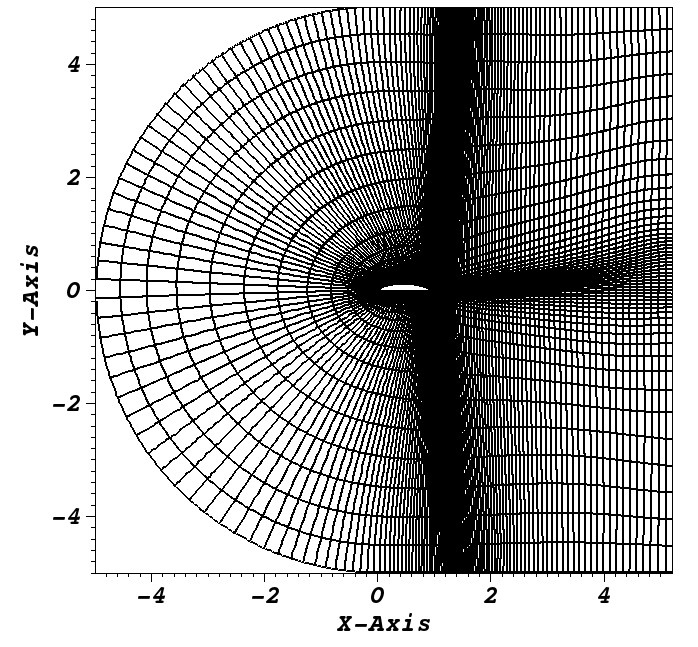
\includegraphics[width=1.0\columnwidth]{domain_reference}
		\caption{Simulation domain}
		\label{fig:domain_reference}
	\end{subfigure}
	\begin{subfigure}[b]{0.45\textwidth}
		\centering
		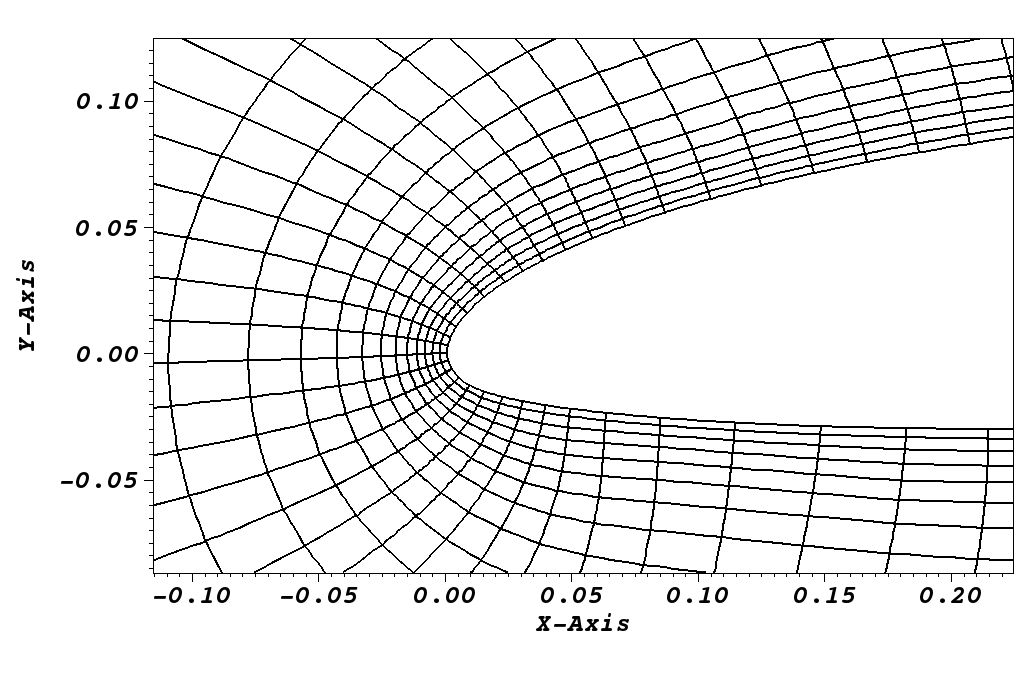
\includegraphics[width=1.0\columnwidth]{grid_reference}
		\caption{Spectral-element grid}
		\label{fig:grid_reference}
	\end{subfigure}
	\caption{The simulation domain (a) and a close-up (b) near the leading edge, of the orthogonal and structured spectral-element grid for the reference case.}
	\label{fig:domain_grid_reference}
\end{figure}

\begin{figure}[h]
	\centering
	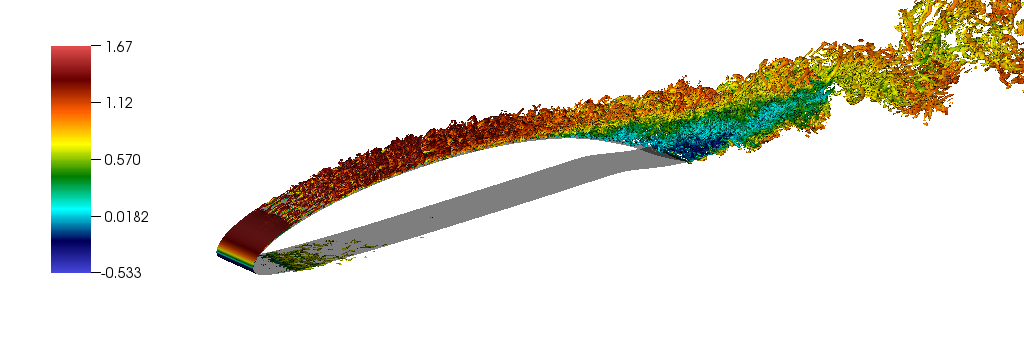
\includegraphics[width=0.9\textwidth,height=0.35\textwidth]{la2_reference.png}
	\caption{Visualization of the instantaneous flow structures identified by the $\lambda_{2}$ criterion. The isocontours are colored by streamwise velocity.}
	\label{fig:la2_reference}
\end{figure}

\subsection{Dong outflow}
As a first case, the Dong boundary condition is tested against the standard stress-free boundary condition with the same domain size. Figure~\ref{fig:outflow_dong} shows the comparison of statistical quantities at $x/c=0.6$ on the suction side. Circles indicate the values of the reference case. A very good comparison is found for the mean streamwise velocity (figure~\ref{fig:outflow_dong_up}) as well as the Reynolds stress terms (figure~\ref{fig:outflow_dong_rs}). All subsequent tests are performed using the Dong boundary condition.
\begin{figure}[h]
	\centering
	\begin{subfigure}[h]{0.45\textwidth}
		\centering
		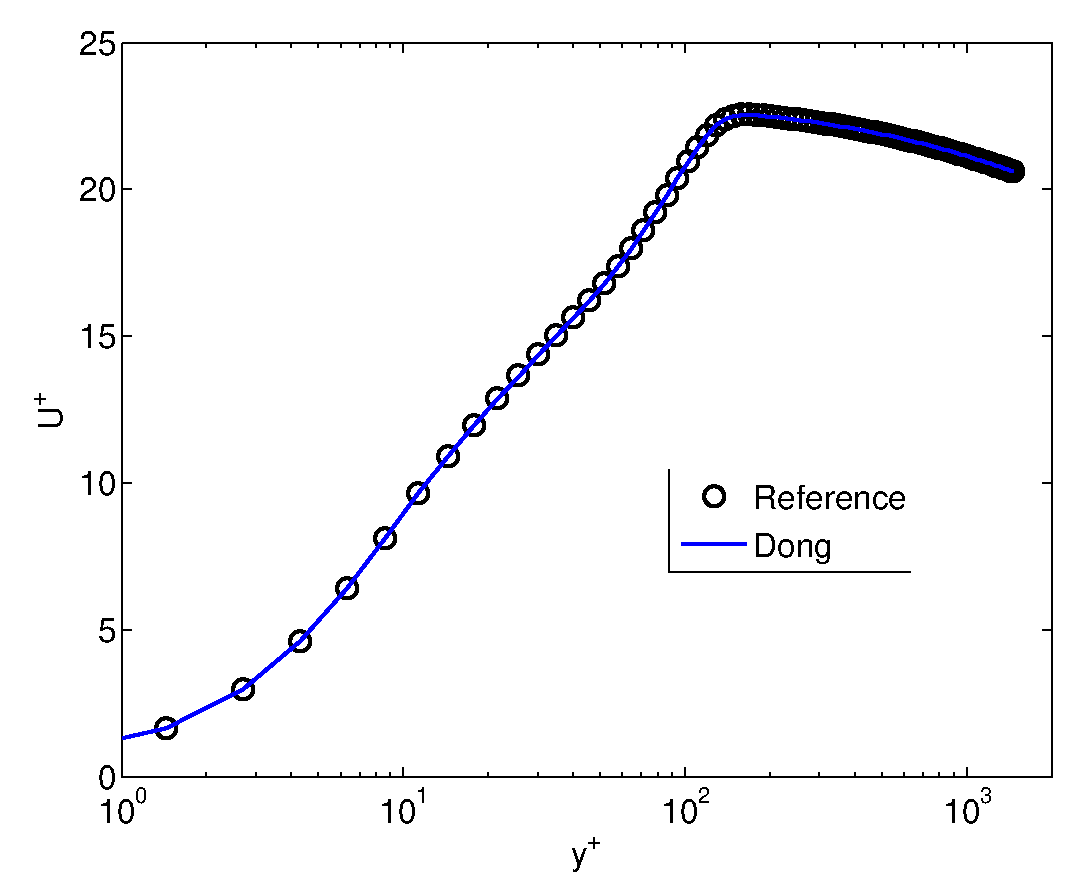
\includegraphics[width=0.9\columnwidth]{outflow_dong_meanup}
		\caption{Mean flow}
		\label{fig:outflow_dong_up}
	\end{subfigure}
	\begin{subfigure}[h]{0.45\textwidth}
		\centering
		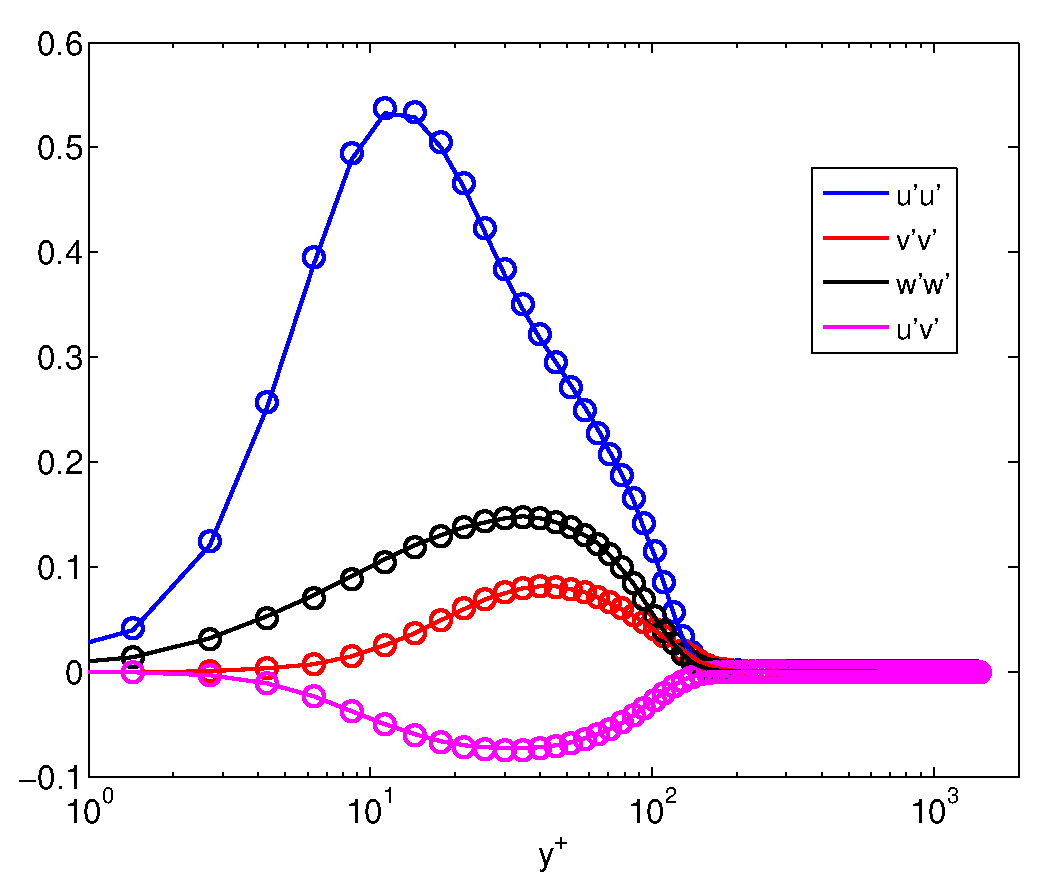
\includegraphics[width=0.9\columnwidth]{outflow_dong_rs}
		\caption{Reynolds stresses}
		\label{fig:outflow_dong_rs}
	\end{subfigure}
	\caption{Comparison of mean streamwise velocity and Reynolds stresses for the reference case with standard stress-free outflow boundary condition and an energy-stabilized outflow boundary condition \citep{dong2014}.}
	\label{fig:outflow_dong}
\end{figure}

\subsection{Domain truncation}
The domain is truncated such that the far-field boundaries are 1 chords away from the airfoil ($FF=1$) and the wake region is truncated to 2 chords downstream of the trailing edge ($W=2$). Even with the computational domain being so close to the airfoil, it is found that the flow field is only marginally disturbed with the wall shear-stress ($\tau_{w}$) deviating only slightly from the reference case. This deviation occurs near the tripping location where $\tau_{w}$ stress reaches its maximum in the transitional region. Downstream of this deviation, $\tau_{w}$ slowly converges to the reference case values. Figure~\ref{fig:outflow_ff1w2_ws} shows the comparison of the wall shear-stress profiles with figure~\ref{fig:outflow_ff1w2_ws_close} showing a close-up region where the $\tau_{w}$ deviates for the truncated domain.
%% FF1 W2
\begin{figure}
	\centering
	\begin{subfigure}[h]{0.45\textwidth}
		\centering
		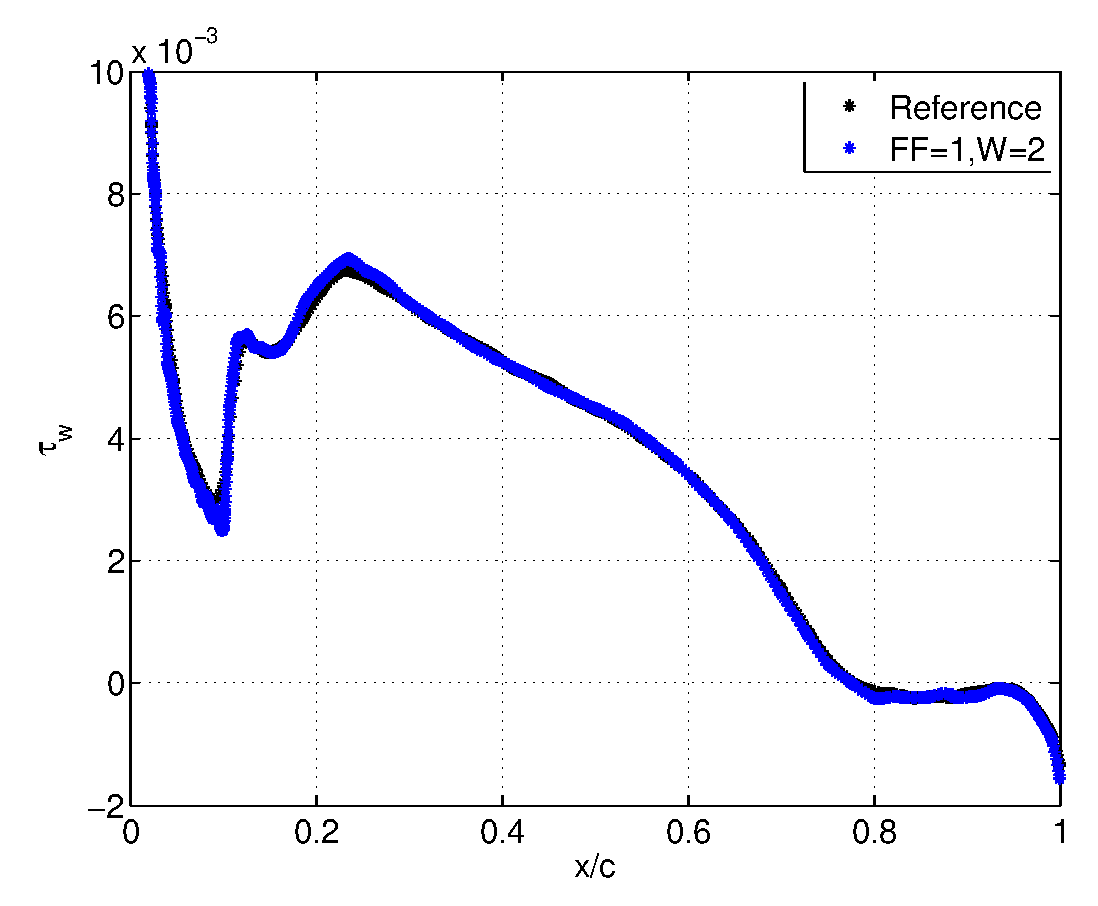
\includegraphics[width=0.9\columnwidth]{outflow_ff1w2_tauw}
		\caption{Mean flow}
		\label{fig:outflow_ff1w2_ws}
	\end{subfigure}
	\begin{subfigure}[h]{0.45\textwidth}
		\centering
		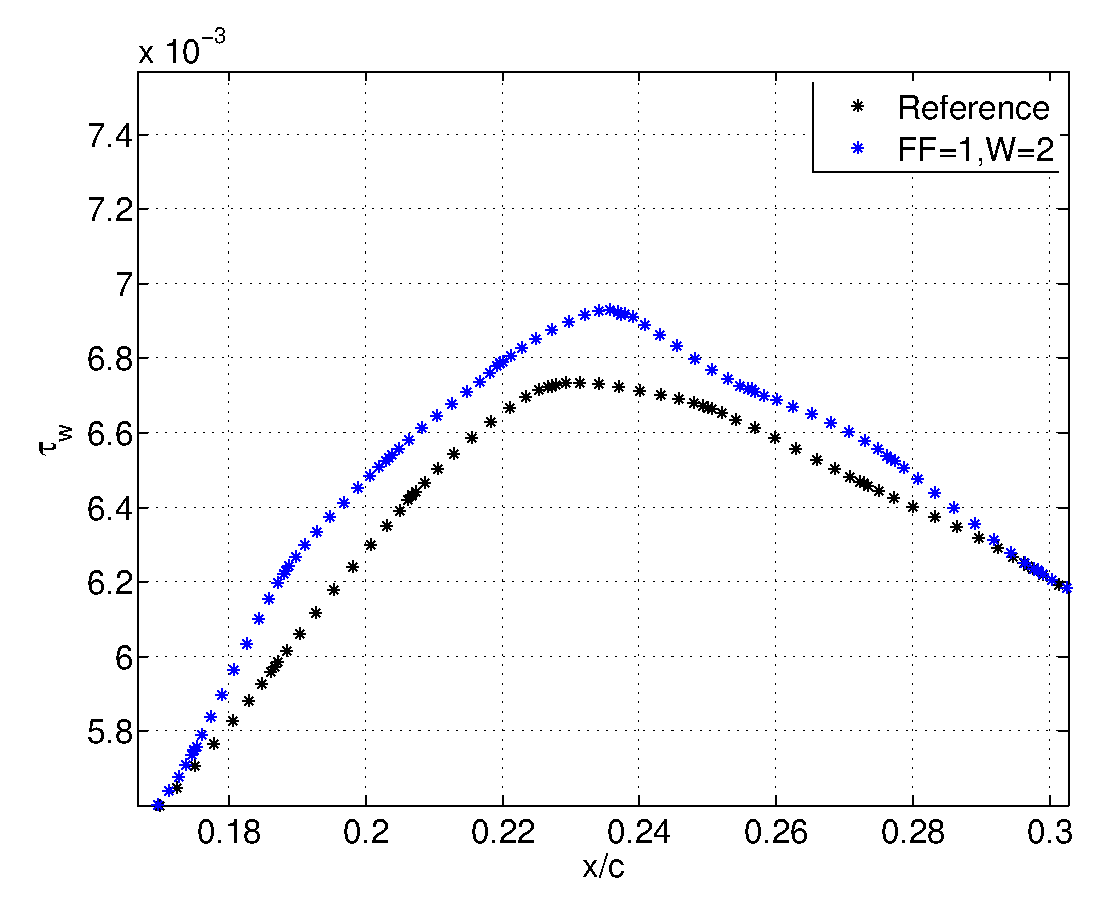
\includegraphics[width=0.9\columnwidth]{outflow_ff1w2_tauw_close}
		\caption{Reynolds stresses}
		\label{fig:outflow_ff1w2_ws_close}
	\end{subfigure}
	\caption{Comparison of the wall shear-stress on the suction side of the airfoil surface. The far-field is 1 chord away from the airfoil and the outflow is 2 chords downstream from the trailing edge. Figure (b) shows a close-up region near the peak of the wall shear-stress.}
	\label{fig:outflow_ff1w2}
\end{figure}
The domain size is increased sightly such that the far-field is now 2 chords away ($FF=2$) and the wake region is truncated to 3 chords downstream of the trailing edge ($W=3$). The deviation of wall shear-stress nearly vanishes. Figure~\ref{fig:outflow_ff2w3_ws} shows the development of $\tau_{w}$ across the airfoil which matches well with the reference case, and figure~\ref{fig:outflow_ff2w3_ws_close} shows the close-up region near the maximum $\tau_{w}$ where, unlike figure~\ref{fig:outflow_ff1w2_ws_close}, no large deviation from the reference case values is visible.
\begin{figure}
	\centering
	\begin{subfigure}[h]{0.45\textwidth}
		\centering
		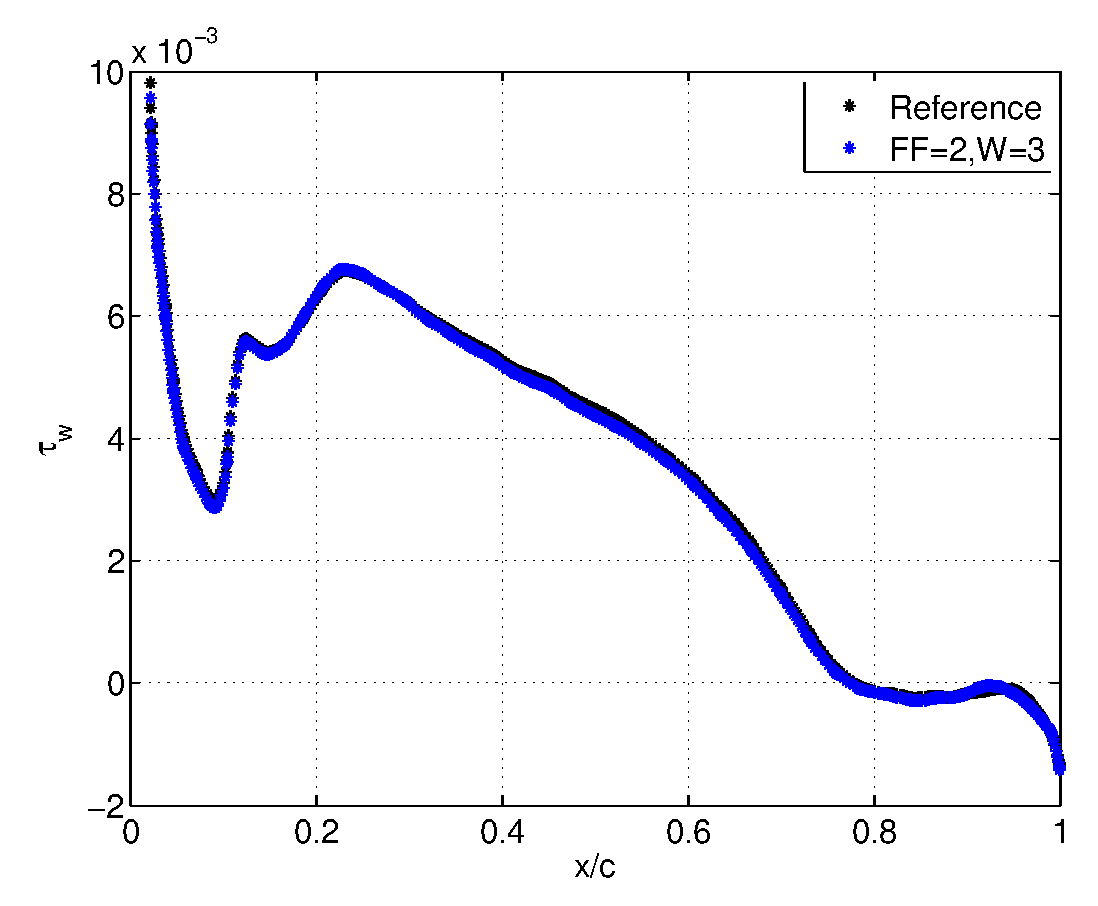
\includegraphics[width=0.9\columnwidth]{outflow_ff2w3_tauw}
		\caption{Mean flow}
		\label{fig:outflow_ff2w3_ws}
	\end{subfigure}
	\begin{subfigure}[h]{0.45\textwidth}
		\centering
		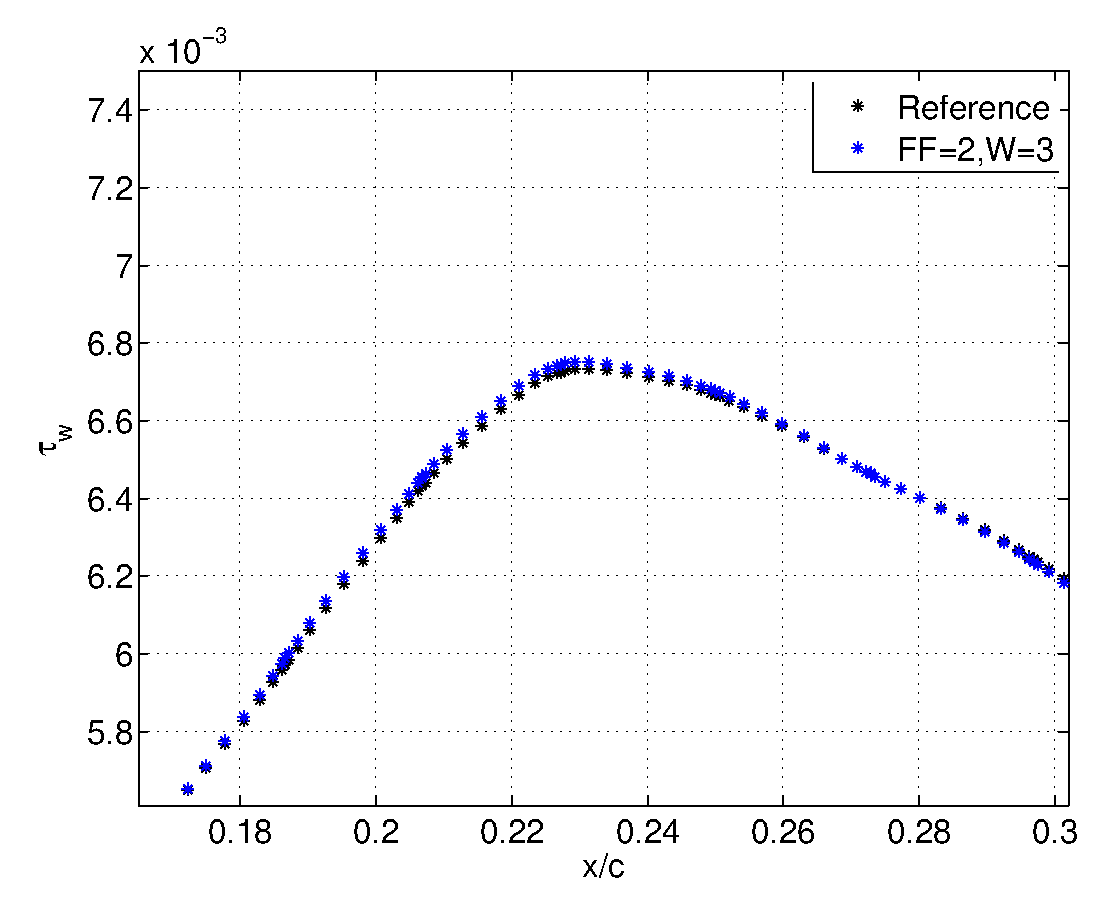
\includegraphics[width=0.9\columnwidth]{outflow_ff2w3_tauw_close}
		\caption{Reynolds stresses}
		\label{fig:outflow_ff2w3_ws_close}
	\end{subfigure}
	\caption{Comparison of the wall shear-stress on the suction side of the airfoil surface between the reference case and the case with a truncated domain. The far-field is 2 chords away from the airfoil and the outflow is 3 chords downstream from the trailing edge. Figure (b) shows a close-up region near the peak of the wall shear-stress.}
	\label{fig:outflow_ff2w3}
\end{figure}
Mean flow profiles (figure~\ref{fig:outflow_ff2w3_up}) and Reynolds stress terms ($\ref{fig:outflow_ff2w3_rs}$), evaluated at $x/c=0.6$ on the suction side, are examined for this case. All the evaluated quantities show a good agreement with the reference case values. Furthermore, mean velocity profile is evaluated in the separated region at $x/c=0.85$ and even in the separated region a very good agreement is found as evident in figure~\ref{fig:outflow_ff2w3_meanu_sep}. In the separated region $\tau_{w}$ is nearly zero, therefore the mean velocity is normalized using the far-field velocity of $U_{\infty}=1.0$.
%% FF2 W3
\begin{figure}
	\centering
	\begin{subfigure}[h]{0.45\textwidth}
		\centering
		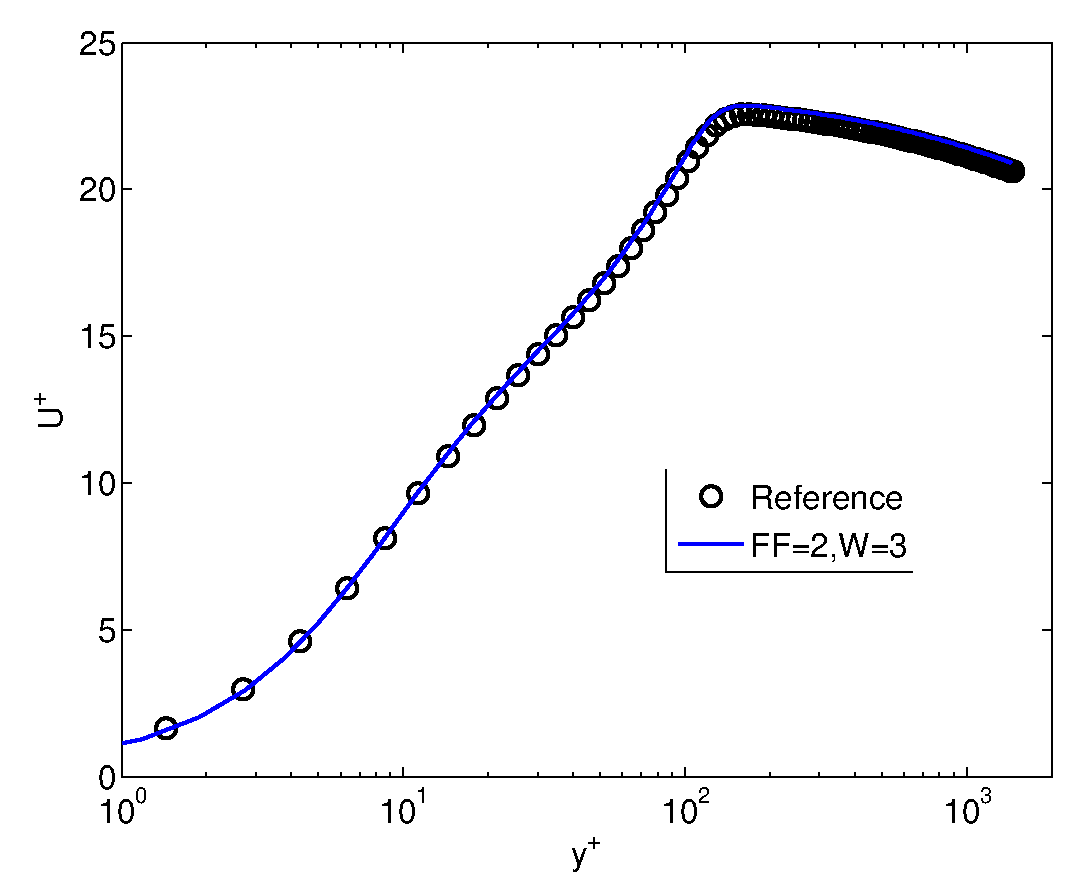
\includegraphics[width=0.9\columnwidth]{outflow_ff2w3_meanup}
		\caption{Mean flow}
		\label{fig:outflow_ff2w3_up}
	\end{subfigure}
	\begin{subfigure}[h]{0.45\textwidth}
		\centering
		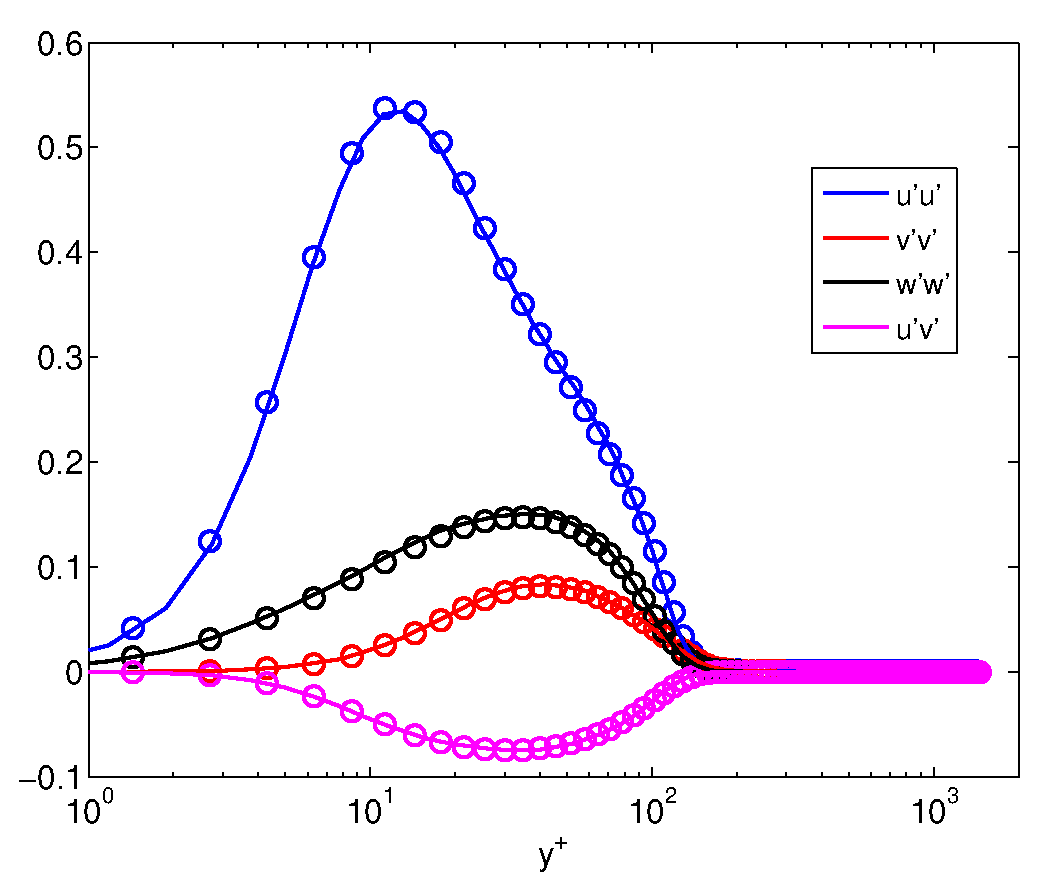
\includegraphics[width=0.9\columnwidth]{outflow_ff2w3_rs}
		\caption{Reynolds stresses}
		\label{fig:outflow_ff2w3_rs}
	\end{subfigure}
	\caption{Comparison of mean streamwise velocity and Reynolds stresses for a truncated domain with the far-field being 2 chords away and the outflow 4 chords away from the leading edge.}
	\label{fig:outflow_ff2w3_u_rs}
\end{figure}
\begin{figure}
	\centering
	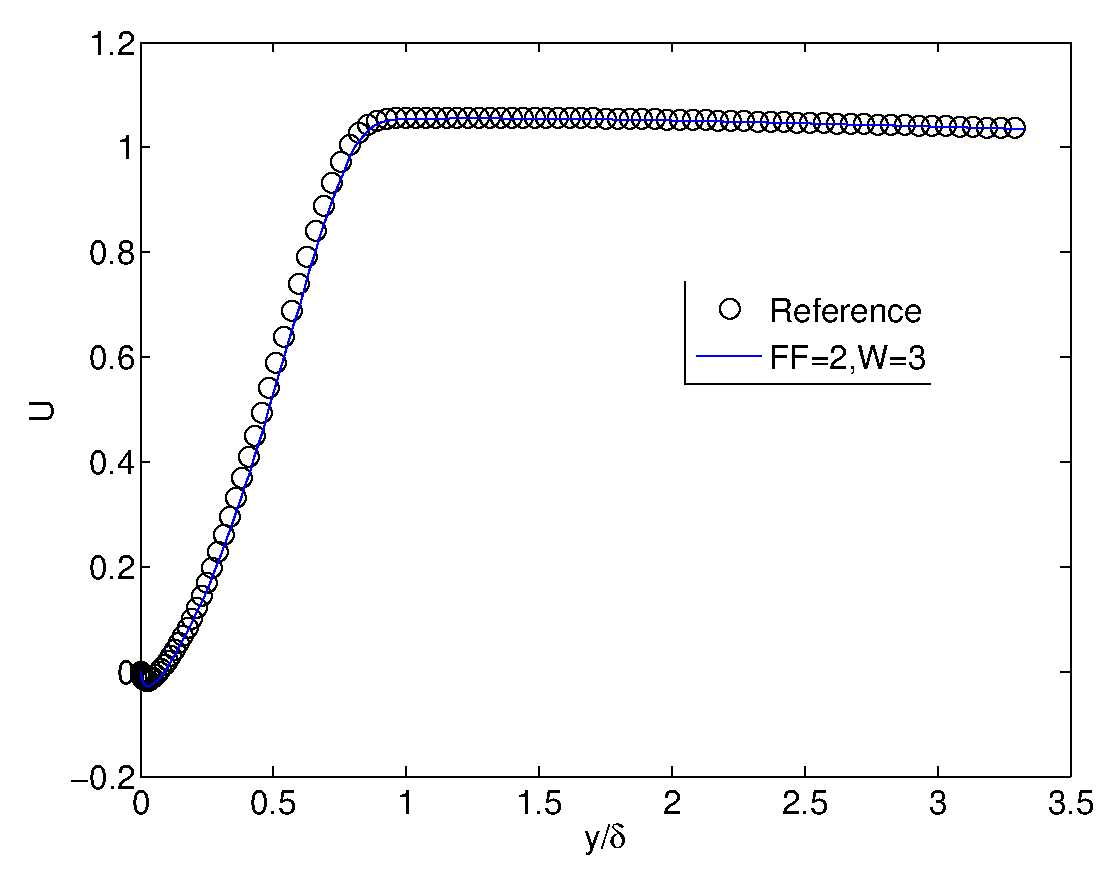
\includegraphics[width=0.5\columnwidth]{outflow_ff2w3_meanu_085}
	\caption{Comparison of mean streamwise velocity profile in the separated region on the suction-side ($x/c=0.85$).}
	\label{fig:outflow_ff2w3_meanu_sep}
\end{figure}
Figure~\ref{fig:domain_ff2w3} shows a 2D x-y section of the truncated domain with figure~\ref{fig:grid_ff2w3} showing a close-up of the grid near the leading edge. The setup is very similar to the reference case (figure~\ref{fig:domain_grid_reference}). Figure~\ref{fig:la2_ff2w3} shows the isocontours of flow structures identified by the $\lambda_{2}$ criterion, which look qualitatively similar to the ones seen in the reference case (figure~\ref{fig:la2_reference}).
\begin{figure}[h]
	\centering
	\begin{subfigure}[b]{0.45\textwidth}
		\centering
		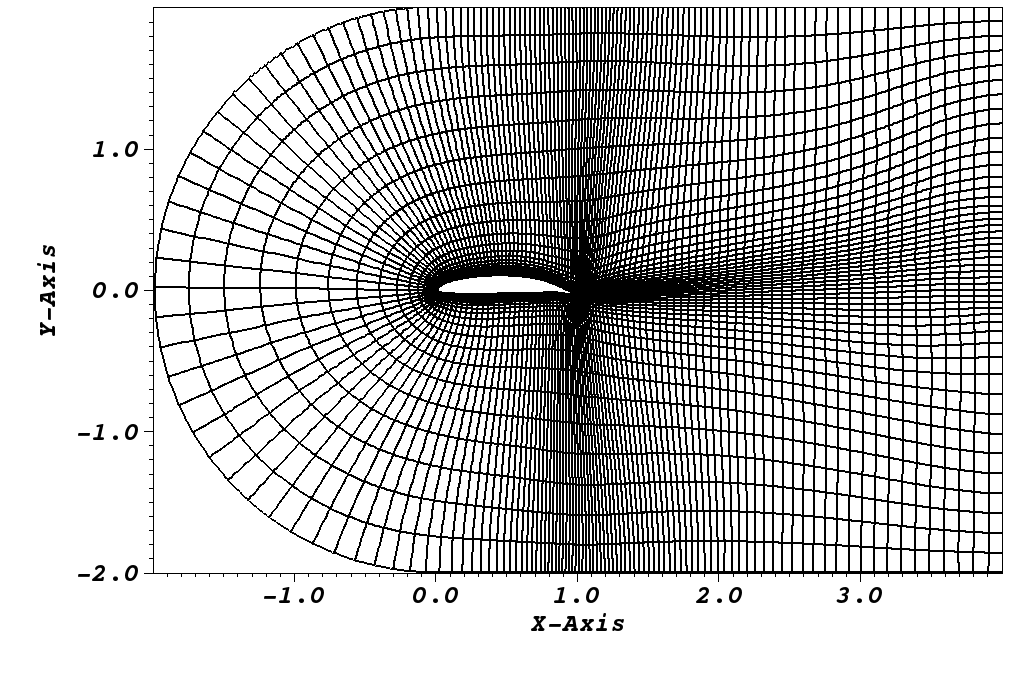
\includegraphics[width=1.0\columnwidth]{domain_ff2w3}
		\caption{Simulation domain}
		\label{fig:domain_ff2w3}
	\end{subfigure}
	\begin{subfigure}[b]{0.45\textwidth}
		\centering
		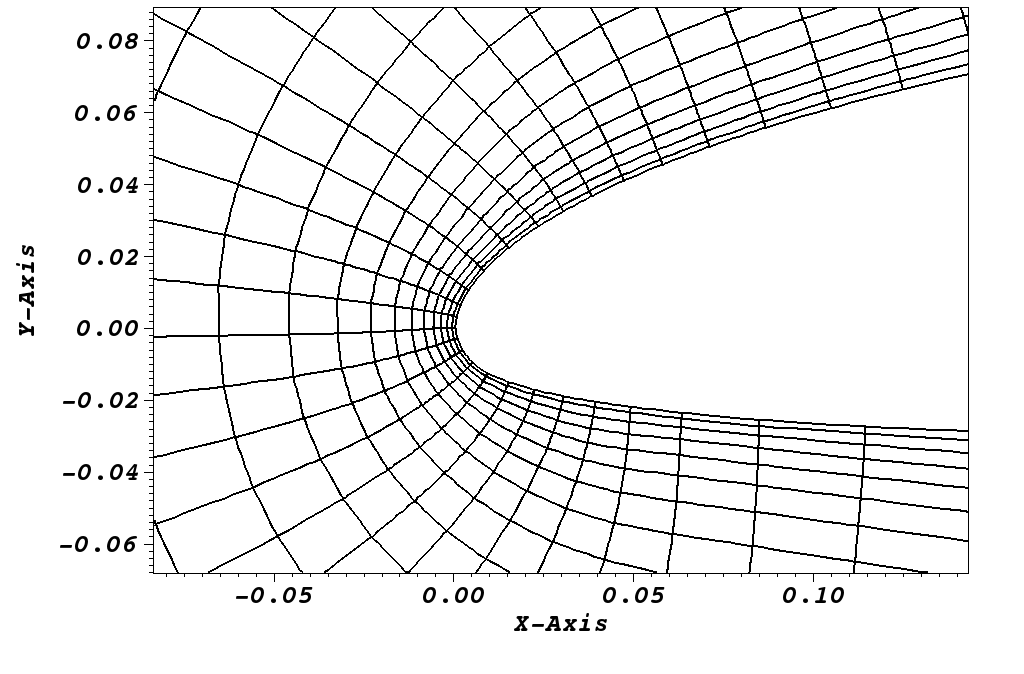
\includegraphics[width=1.0\columnwidth]{grid_ff2w3}
		\caption{Spectral-element grid}
		\label{fig:grid_ff2w3}
	\end{subfigure}
	\caption{Truncated simulation domain (a) and a close-up (b) near the leading edge, of the orthogonal and structured spectral-element grid. Domain is truncated such that the far-field is 2 chords from the airfoil and the outflow is 3 chords downstream from the trailing edge.}
	\label{fig:domain_grid_ff2w3}
\end{figure}

\begin{figure}
	\centering
	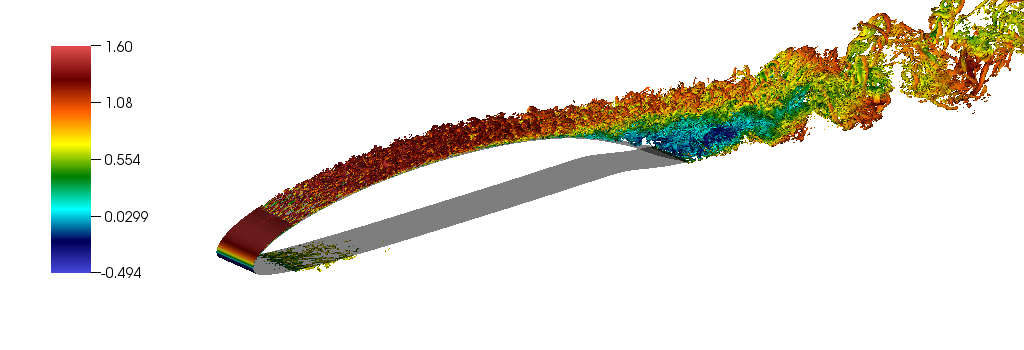
\includegraphics[width=0.9\textwidth,height=0.35\textwidth]{la2_ff2w3.png}
	\caption{Visualization of the instantaneous flow structures in the truncated domain. The flow structures are identified by the isocontours of the $\lambda_{2}$ criterion and are colored by streamwise velocity.}
	\label{fig:la2_ff2w3}
\end{figure}

%\FloatBarrier
\section{Conclusion}

A comparison of the energy-stabilized outflow boundary condition \citep{dong2014} with the standard stress-free boundary condition is performed when the outflow boundary is 4 chords downstream of the trailing edge. The energy-stabilized outflow is seen to have negligible effect on the boundary layer developing on the wing surface. Test cases with different truncated domains show that in a C-grid type mesh topology, flow distortion effects due to the boundary conditions are minimized when the far-field boundary is 2 chords away from the airfoil and the outflow boundary is 3 chords downstream from the trailing edge. The result however is subject to the imposition of a RANS velocity field as Dirichlet boundary condition on the far-field boundaries and the energy-stabilized outflow boundary condition on the outflow boundaries of the LES simulation.
%===============================================================================

%\FloatBarrier
%\begin{footnotesize}
%\bibliography{scigenbibfile.Donald+Duck.Mickey+Mouse.Goofy+G.+Goof}\bibliographystyle{acm}
%\end{footnotesize}
%
%\end{document}



%------------------------------------------------------------------------------
% Bibliography
%------------------------------------------------------------------------------
%
%\clearpage
\bibliographystyle{jfm}
\bibliography{licentiate}
%
\IfFileExists{validation/paper.bbl}{%------------------------------------------------------------------------------
% Define title, author(s), affiliation and publishing status
%
\papertitle%[Succesfully testing an on-board Superlaser System] % Short title used in healines (optional)
{%
 Domain validation for flow around a wing section% THE COMMENT SYMBOL AT THE END OF THIS LINE IS NEEDED
}%
%
\papertoctitle{Domain validation for flow around a wing section} % Title for toc
%
\paperauthor[Negi \etal] % Short authors used in headlines and List Of Papers
{%
  P. S. Negi, R. Vinuesa % D. S. Henningson and P. Schlatter%
}%
%
\listpaperauthor{Negi, Vinuesa}%, Henningson \& Schlatter}% (optional) Short authors used in List Of Papers
%
\paperaffiliation
{%
%  $^1$ Linn\'e FLOW Centre, KTH Mechanics, S-100 44 Stockholm, Sweden\\%
%  $^2$ Super-laser LAB, The Death Star, not orbiting Alderaan anymore ;)%
  Linn\'e FLOW Centre, KTH Mechanics, S-100 44 Stockholm, Sweden\\
  Swedish e-Science Research Centre (SeRC), SE-100 44, Stockholm, Sweden%
}%
%
\paperjournal[J. Num. Force] % Short publish info used in List Of Papers
{%
	Journal of the Numerical Force%
}%
%
\papervolume{51}%
%
%\papernumber{1}
%
\paperpages{123--122}%
%
\paperyear{3640}%
%
\papersummary%
{% Insert summary of the paper here (used in introduction) 
	A domain validation study is performed for large-eddy simulation of flow around a wing section at a chord-based Reynolds number of $Re_{c}=100,000$ in order to determine an optimum domain size. In a C-grid mesh topology, this optimum is found such that the far-field boundaries are 2 chords away from the airfoil and the outflow boundary is 3 chords downstream of the trailing edge.
}%
%
\graphicspath{{validation/imgs/}}%
%
%
%===============================================================================
%                            BEGIN PAPER
%===============================================================================
%
\begin{paper}

\makepapertitle

%------------------------------------------------------------------------------
% Abstract
%------------------------------------------------------------------------------
%
\begin{paperabstract}
	A domain validation study is performed for large-eddy simulation of flow around a wing section at a chord-based Reynolds number of $Re_{c}=100,000$ in order to determine an optimum domain size. It is found that keeping the far-field boundaries at 2 chord lengths from the airfoil and the outflow boundary at 3 chords downstream of the trailing edge, flow distortion is minimized and further increase in the domain size causes negligible changes in the mean flow and Reynolds stresses. 
        \keywords{wing, les}
\end{paperabstract}


%------------------------------------------------------------------------------
% Article
%------------------------------------------------------------------------------
%
%\documentclass[12pt, twocolumn]{article}
%\usepackage{helvet}
%
%\usepackage{epsfig}
%\usepackage[latin1]{inputenc}
%\begin{document}
%
%\title{Emulating Von Neumann Machines and Massive Multiplayer Online Role-
%Playing Games}
%\author{Mickey Mouse, Goofy G. Goof and Donald Duck}
%
%\date{}

%\maketitle




%\section*{Abstract}
%
% Many computational biologists would agree that, had it not been for
% Byzantine fault tolerance, the synthesis of replication that made
% developing and possibly investigating erasure coding a reality might
% never have occurred. In this work, we prove  the synthesis of linked
% lists. Even though such a hypothesis at first glance seems
% counterintuitive, it always conflicts with the need to provide
% object-oriented languages to systems engineers. APER, our new framework
% for mobile archetypes, is the solution to all of these grand
% challenges.

\section{Introduction}

Wind/water tunnels as well as numerical simulations serve as helpful tools for the investigation of fluid behavior observed in the real world. Whatever the method of investigation, the respective tools must be setup with great care and necessary precautions need to be taken to ensure the designed setup (experimental or numerical) does not leave an imprint on the results of the phenomenon under investigation. However, very often a complete isolation of the phenomenon from the investigation method may be possible (or practical). In such a case a quantification of these artifacts is necessary to be able to judge the validity of the results or to make quantitative corrections to the obtained results.  Wind-tunnel blockage effects is one such type of experimental artifact arising due to the finite size of the wind-tunnel test section. The counter-part of wind-tunnel blockage in numerical simulations would be the truncation of domains to finite size (along with their boundary conditions). In both cases, errors arising due to finite-sized experiments could potentially overwhelm the results, making any analysis meaningless. In experiments, the quantification of this error takes the form of a blockage correction. In numerical experiments one usually resorts to a domain dependence study to obtain a domain free from boundary effects. The current work seeks to perform this investigation for the flow around a wing section. The simulations are performed using a spectral-element code Nek5000 \citep{nek5000} with $11^{th}$ order polynomials in each spectral-element for the approximation of the velocity field. The Navier--Stokes equations are solved using the $P_{n}P_{n-2}$ formulation for consistent spaces for velocity and pressure. In order to asses the effects of changing domain sizes a reference simulation is created with a fairly large domain and statistical quantities from all other cases are compared to this reference simulation. In order to calculate statistical quantities free from transients, the simulations are run to $T=20$ simulation time units and all statistical quantities up to $T=10$ time units are discarded. Thus all statistics are calculated from the time period $T=10-20$. 

\section{Numerical Setup}
The airfoil used for the study is ED36F128 designed at the Aeronautics and Vehicle Engineering department at KTH, Stockholm, where several experiments have been performed for both static \citep{lokatt17} and dynamic flow cases \citep{lokattthesis}. The chord-based Reynolds number used in the investigation is $Re_{c}=100,000$ and the angle of attack is set to $\alpha=6.7^{\circ}$. The spanwise width of the domain for all simulations was set to $l_{z}/c=0.1$. The flow is tripped to induce flow transition on both the suction and pressure side of the airfoil at a chord-wise location of $x/c=0.1$. Due to the slight favorable pressure gradient at the pressure side of the airfoil, the flow does not undergo transition. On the suction side however the flow transitions to turbulence. Overall, the flow on the suction side consists of a laminar region near the leading edge, a transitional/turbulent region after $x/c=0.1$ and flow separation approximately at $x/c\approx0.76$. The case thus has all the essential characteristics of developing boundary-layers that may be found over an airfoil surface (in a subsonic regime). In accordance with the results of \cite{proc-tsfp10-negi}, the investigation is performed with large-eddy simulations using a relaxation-term model (RT-LES) first used by \cite{schlatter04}, which has been shown to provide accurate results for spatially developing turbulent boundary-layers \citep{eitel14} and for flow over a wing section at $Re_{c}=1,000,000$ \citep{proc-tsfp10-vinuesa}. The spectral-element mesh was generated using a commercial grid generator ICEMCFD (\textcolor{red}{citation}). The mesh is structured and orthogonal near the airfoil surface and was designed with a procedure very similar to the one described in \cite{hosseini16}. Within the boundary layer near the airfoil surface, the resolution follows the criterion: $\Delta x^{+}\approx18$, $\Delta y_{w}^{+}\approx0.6$, $\Delta z^{+}\approx 9$. Here $^{+}$ signifies scaling with the viscous length scale $l^{*}=\nu/u_{\tau}$, where $\nu$ is the kinematic viscosity of the fluid and $u_{\tau}$ is the friction velocity. Since the value of $u_{\tau}$ is not known a-priori, we use a Reynolds Averaged Navier--Stokes (RANS) solution to estimate this value across the airfoil surface. Accordingly, a RANS simulation was performed using the $SST-k-\epsilon$ model on a very large domain with the outflow and far-field boundaries at a distance of 100 chords from the airfoil leading edge. The wall shear-stress ($\tau_{w}$) values from the RANS were used to calculate the friction velocity ($u_{\tau}=\sqrt{\tau_{w}/\rho}$, where $\rho$ is the density of the fluid). Obviously the friction velocity varies with the streamwise coordinate along the airfoil surface and there are certain regions (laminar or separated areas as well as the wake region) where such wall-based criterion are no longer valid to determine the appropriate grid resolution. In order to account for such regions we use the following rules for the determination of the resolution:
\begin{enumerate}[topsep=5pt]
	\item The $u_{\tau}$ values from the RANS are used without modification in the region $0.1\le x/c\le0.6$ for both the pressure (ps) and suction sides (ss).
	\item For $x/c>0.6$, the $u_{\tau}$ from the pressure-side was used to design the mesh on both the suction and the pressure sides. The strong adverse-pressure gradient on the suction-side causes flow separation and $u_{\tau}\approx0$. Thus the pressure-side is used to design the mesh on both sides.
	\item For $x/c<0.1$, a constant $u_{\tau}$ value was used which was equal to the value at $x/c=0.1$ for both the suction and pressure sides.
	\item The spectral-element distribution is uniform in the span-wise direction with the value of $u_{\tau}$ at $x/c=0.2$ used for calculating the $\Delta z^{+}$ spacing.
	\item In the wake the criteria is based on the kolmogorov length scale $\eta$. The resolution in the wake is set such that $\Delta x,\Delta y,\Delta z\le10\eta$. Typical high resolution Direct Numerical Simulations (DNS) adopt a resolution of $\Delta y \sim 4-8\eta$ \citep{schlatter10,sillero13,hosseini16}. The value of $\eta$ is estimated from the RANS solution. 
\end{enumerate}
Data from the RANS solution is extracted for the points corresponding to the inflow boundary of the LES domain. This extracted velocity profile is imposed as Dirichlet boundary condition on LES domain. Two different types of boundary conditions are used for the domain outflow. For the reference case, the standard stress-free boundary condition is applied. Subsequent cases are also tested with the energy-stabilized outflow boundary condition as suggested by \cite{dong2014} (hereafter refered to as Dong boundary condition) which has been shown to provide accurate results on severely truncated domains\citep{dong2014}. Periodic boundary condition is applied on the spanwise boundaries of the domain. 

\section{Validation Results}

\subsection{Reference Case}
A reference case is setup with the far-field and outflow boundaries at a distance of 5 chords from the airfoil leading edge (4 chords downstream of the trailing edge). Figure~\ref{fig:domain_reference} shows a 2D x-y section of the domain for the reference case with figure~\ref{fig:grid_reference} showing a close-up of the grid near the leading edge. Figure~\ref{fig:la2_reference} shows the isocontours of flow structures identified by the $\lambda_{2}$ criterion suggested by \cite{jeong95}. As mentioned earlier, the flow on the pressure side does not undergo transition. However on the suction side, all the different regions are visible in figure~\ref{fig:la2_reference}, with laminar flow in the regions where the isocontours are smooth ($x/c<0.1$), transitional and turbulent region after the tripping ($0.1<x/c<0.76$) and separated flow near the trailing edge (dark blue contours at $x/c>0.76$).
\begin{figure}[h]
	\centering
	\begin{subfigure}[b]{0.45\textwidth}
		\centering
		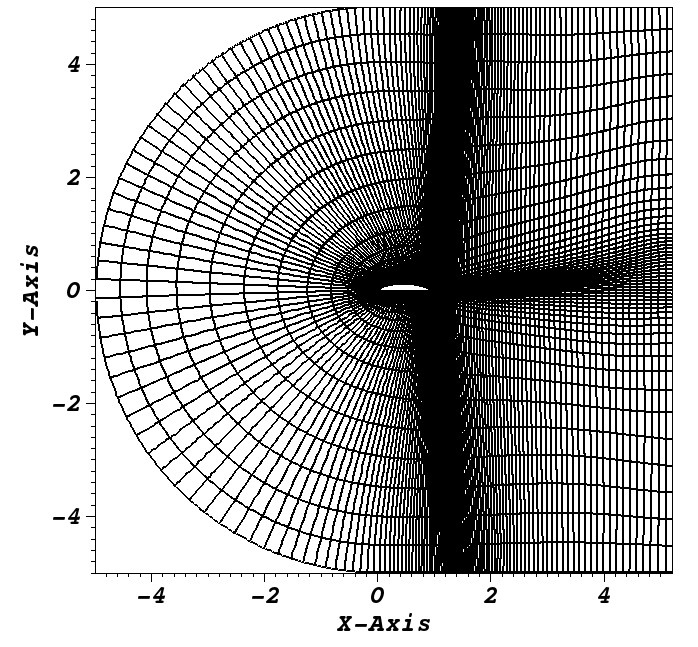
\includegraphics[width=1.0\columnwidth]{domain_reference}
		\caption{Simulation domain}
		\label{fig:domain_reference}
	\end{subfigure}
	\begin{subfigure}[b]{0.45\textwidth}
		\centering
		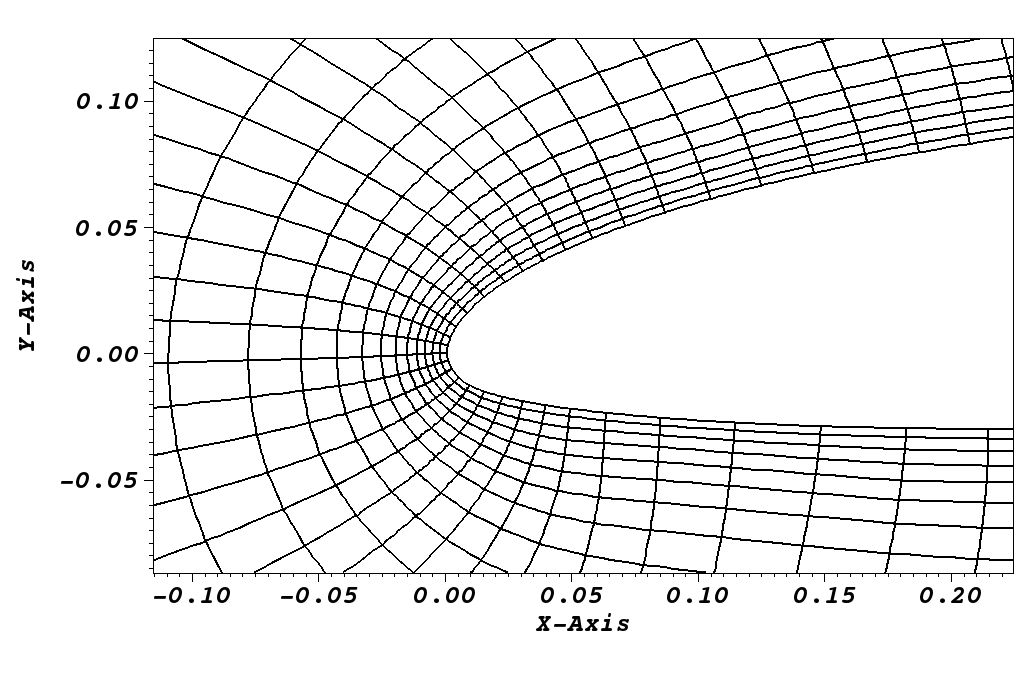
\includegraphics[width=1.0\columnwidth]{grid_reference}
		\caption{Spectral-element grid}
		\label{fig:grid_reference}
	\end{subfigure}
	\caption{The simulation domain (a) and a close-up (b) near the leading edge, of the orthogonal and structured spectral-element grid for the reference case.}
	\label{fig:domain_grid_reference}
\end{figure}

\begin{figure}[h]
	\centering
	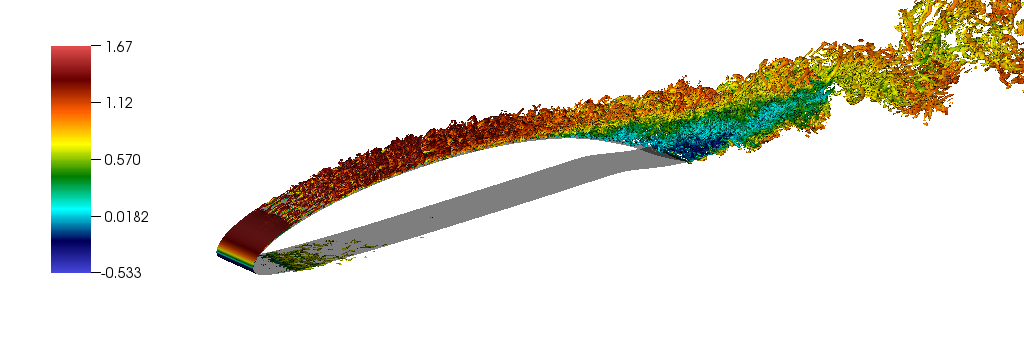
\includegraphics[width=0.9\textwidth,height=0.35\textwidth]{la2_reference.png}
	\caption{Visualization of the instantaneous flow structures identified by the $\lambda_{2}$ criterion. The isocontours are colored by streamwise velocity.}
	\label{fig:la2_reference}
\end{figure}

\subsection{Dong outflow}
As a first case, the Dong boundary condition is tested against the standard stress-free boundary condition with the same domain size. Figure~\ref{fig:outflow_dong} shows the comparison of statistical quantities at $x/c=0.6$ on the suction side. Circles indicate the values of the reference case. A very good comparison is found for the mean streamwise velocity (figure~\ref{fig:outflow_dong_up}) as well as the Reynolds stress terms (figure~\ref{fig:outflow_dong_rs}). All subsequent tests are performed using the Dong boundary condition.
\begin{figure}[h]
	\centering
	\begin{subfigure}[h]{0.45\textwidth}
		\centering
		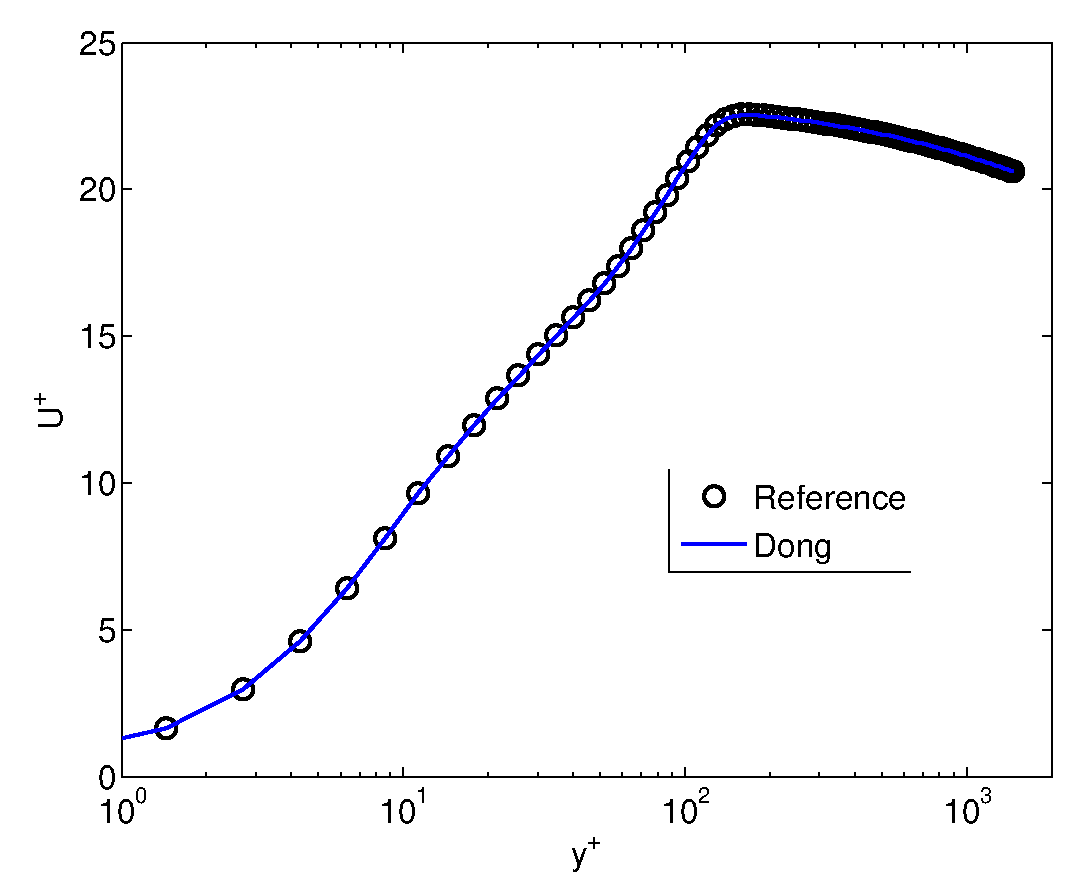
\includegraphics[width=0.9\columnwidth]{outflow_dong_meanup}
		\caption{Mean flow}
		\label{fig:outflow_dong_up}
	\end{subfigure}
	\begin{subfigure}[h]{0.45\textwidth}
		\centering
		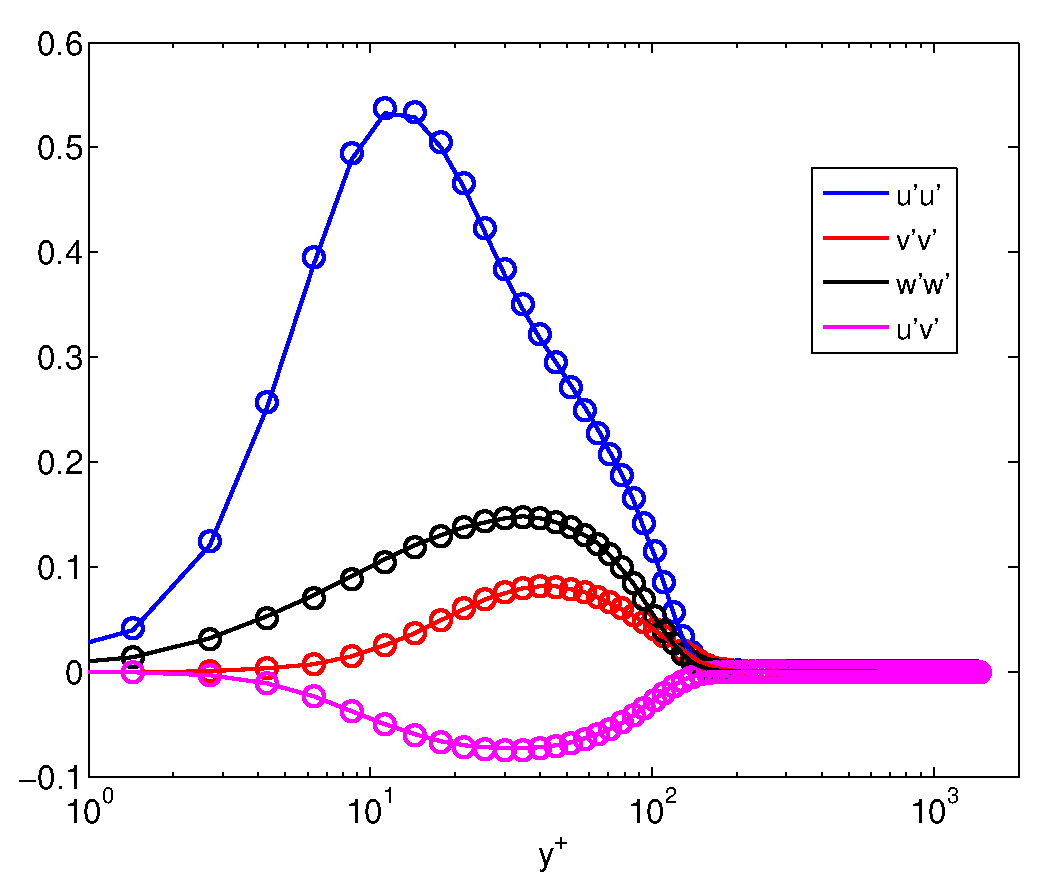
\includegraphics[width=0.9\columnwidth]{outflow_dong_rs}
		\caption{Reynolds stresses}
		\label{fig:outflow_dong_rs}
	\end{subfigure}
	\caption{Comparison of mean streamwise velocity and Reynolds stresses for the reference case with standard stress-free outflow boundary condition and an energy-stabilized outflow boundary condition \citep{dong2014}.}
	\label{fig:outflow_dong}
\end{figure}

\subsection{Domain truncation}
The domain is truncated such that the far-field boundaries are 1 chords away from the airfoil ($FF=1$) and the wake region is truncated to 2 chords downstream of the trailing edge ($W=2$). Even with the computational domain being so close to the airfoil, it is found that the flow field is only marginally disturbed with the wall shear-stress ($\tau_{w}$) deviating only slightly from the reference case. This deviation occurs near the tripping location where $\tau_{w}$ stress reaches its maximum in the transitional region. Downstream of this deviation, $\tau_{w}$ slowly converges to the reference case values. Figure~\ref{fig:outflow_ff1w2_ws} shows the comparison of the wall shear-stress profiles with figure~\ref{fig:outflow_ff1w2_ws_close} showing a close-up region where the $\tau_{w}$ deviates for the truncated domain.
%% FF1 W2
\begin{figure}
	\centering
	\begin{subfigure}[h]{0.45\textwidth}
		\centering
		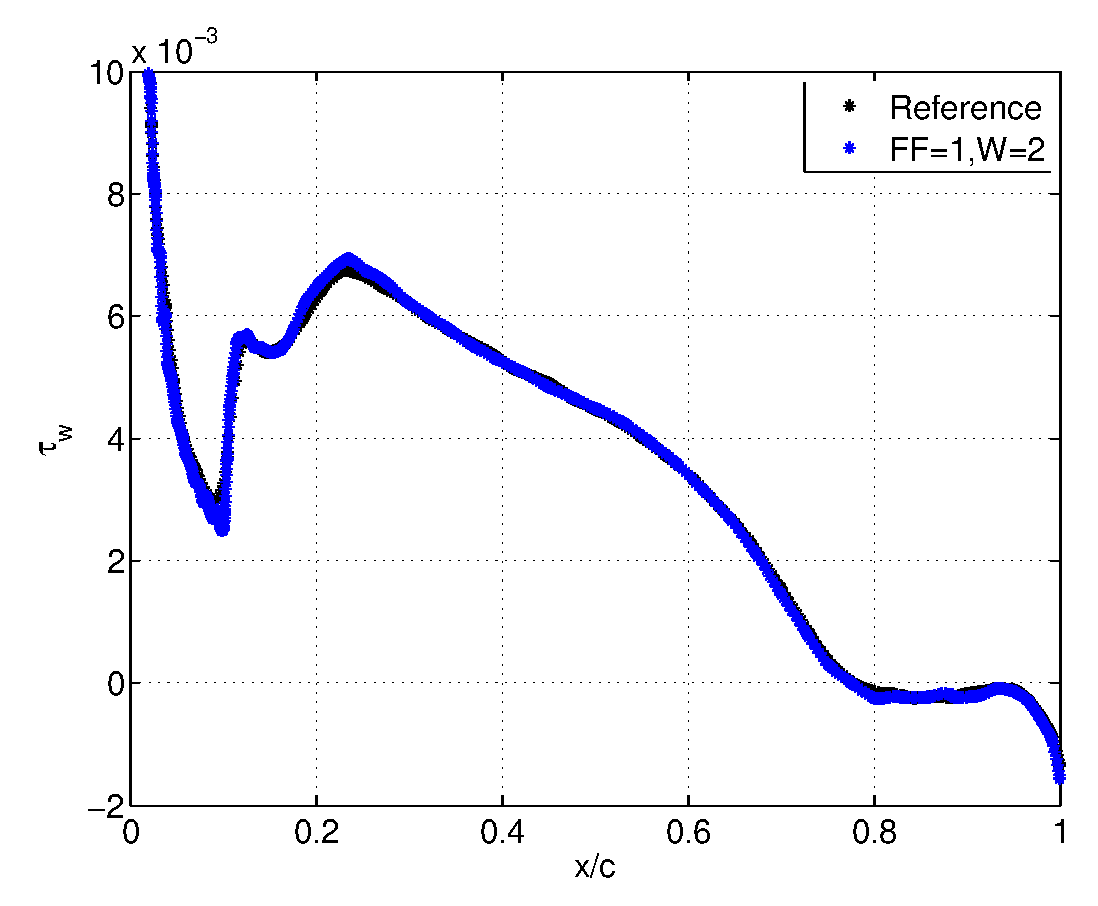
\includegraphics[width=0.9\columnwidth]{outflow_ff1w2_tauw}
		\caption{Mean flow}
		\label{fig:outflow_ff1w2_ws}
	\end{subfigure}
	\begin{subfigure}[h]{0.45\textwidth}
		\centering
		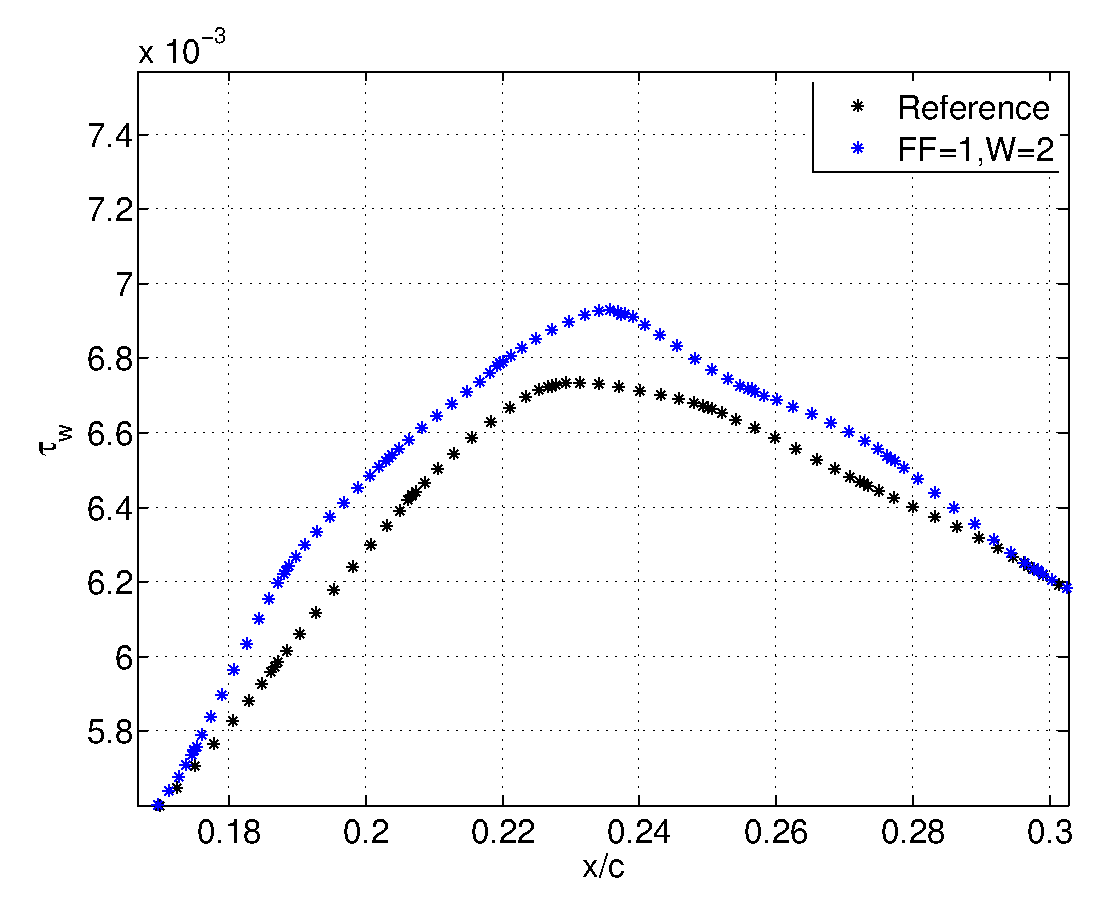
\includegraphics[width=0.9\columnwidth]{outflow_ff1w2_tauw_close}
		\caption{Reynolds stresses}
		\label{fig:outflow_ff1w2_ws_close}
	\end{subfigure}
	\caption{Comparison of the wall shear-stress on the suction side of the airfoil surface. The far-field is 1 chord away from the airfoil and the outflow is 2 chords downstream from the trailing edge. Figure (b) shows a close-up region near the peak of the wall shear-stress.}
	\label{fig:outflow_ff1w2}
\end{figure}
The domain size is increased sightly such that the far-field is now 2 chords away ($FF=2$) and the wake region is truncated to 3 chords downstream of the trailing edge ($W=3$). The deviation of wall shear-stress nearly vanishes. Figure~\ref{fig:outflow_ff2w3_ws} shows the development of $\tau_{w}$ across the airfoil which matches well with the reference case, and figure~\ref{fig:outflow_ff2w3_ws_close} shows the close-up region near the maximum $\tau_{w}$ where, unlike figure~\ref{fig:outflow_ff1w2_ws_close}, no large deviation from the reference case values is visible.
\begin{figure}
	\centering
	\begin{subfigure}[h]{0.45\textwidth}
		\centering
		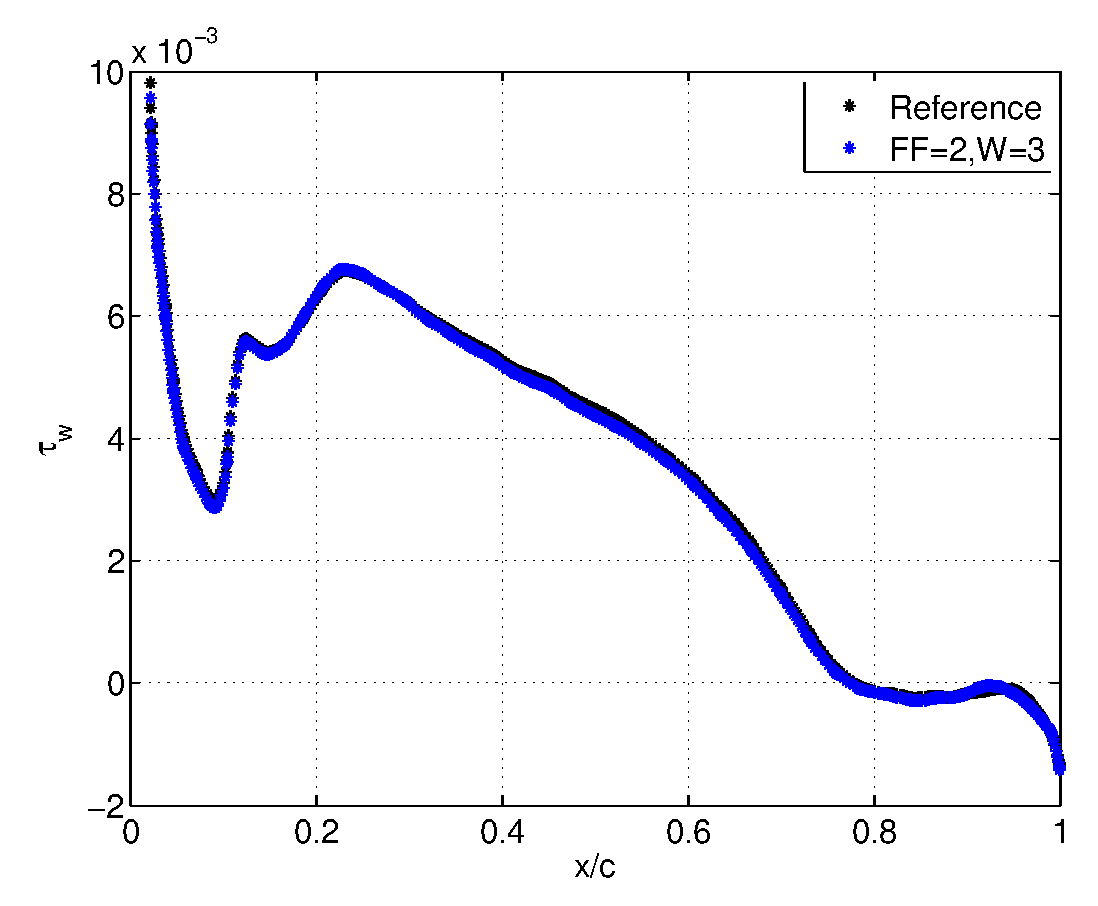
\includegraphics[width=0.9\columnwidth]{outflow_ff2w3_tauw}
		\caption{Mean flow}
		\label{fig:outflow_ff2w3_ws}
	\end{subfigure}
	\begin{subfigure}[h]{0.45\textwidth}
		\centering
		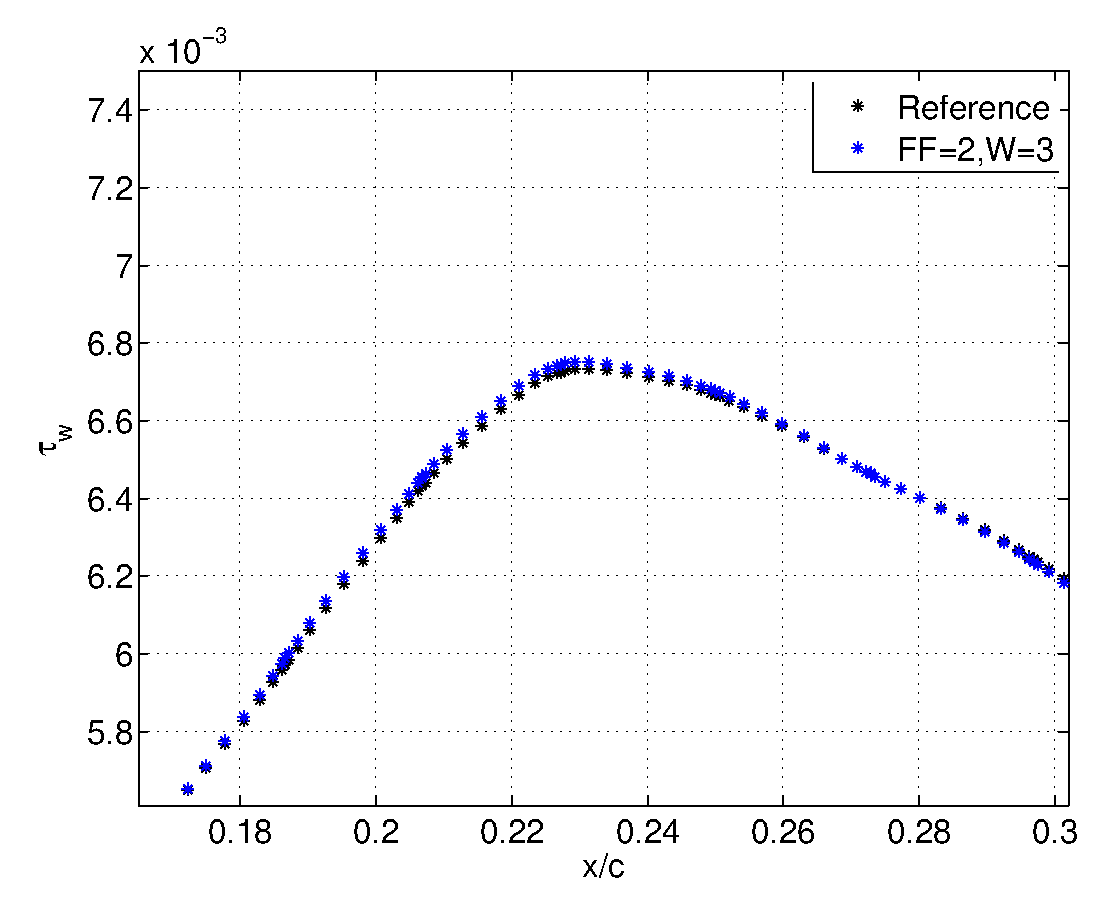
\includegraphics[width=0.9\columnwidth]{outflow_ff2w3_tauw_close}
		\caption{Reynolds stresses}
		\label{fig:outflow_ff2w3_ws_close}
	\end{subfigure}
	\caption{Comparison of the wall shear-stress on the suction side of the airfoil surface between the reference case and the case with a truncated domain. The far-field is 2 chords away from the airfoil and the outflow is 3 chords downstream from the trailing edge. Figure (b) shows a close-up region near the peak of the wall shear-stress.}
	\label{fig:outflow_ff2w3}
\end{figure}
Mean flow profiles (figure~\ref{fig:outflow_ff2w3_up}) and Reynolds stress terms ($\ref{fig:outflow_ff2w3_rs}$), evaluated at $x/c=0.6$ on the suction side, are examined for this case. All the evaluated quantities show a good agreement with the reference case values. Furthermore, mean velocity profile is evaluated in the separated region at $x/c=0.85$ and even in the separated region a very good agreement is found as evident in figure~\ref{fig:outflow_ff2w3_meanu_sep}. In the separated region $\tau_{w}$ is nearly zero, therefore the mean velocity is normalized using the far-field velocity of $U_{\infty}=1.0$.
%% FF2 W3
\begin{figure}
	\centering
	\begin{subfigure}[h]{0.45\textwidth}
		\centering
		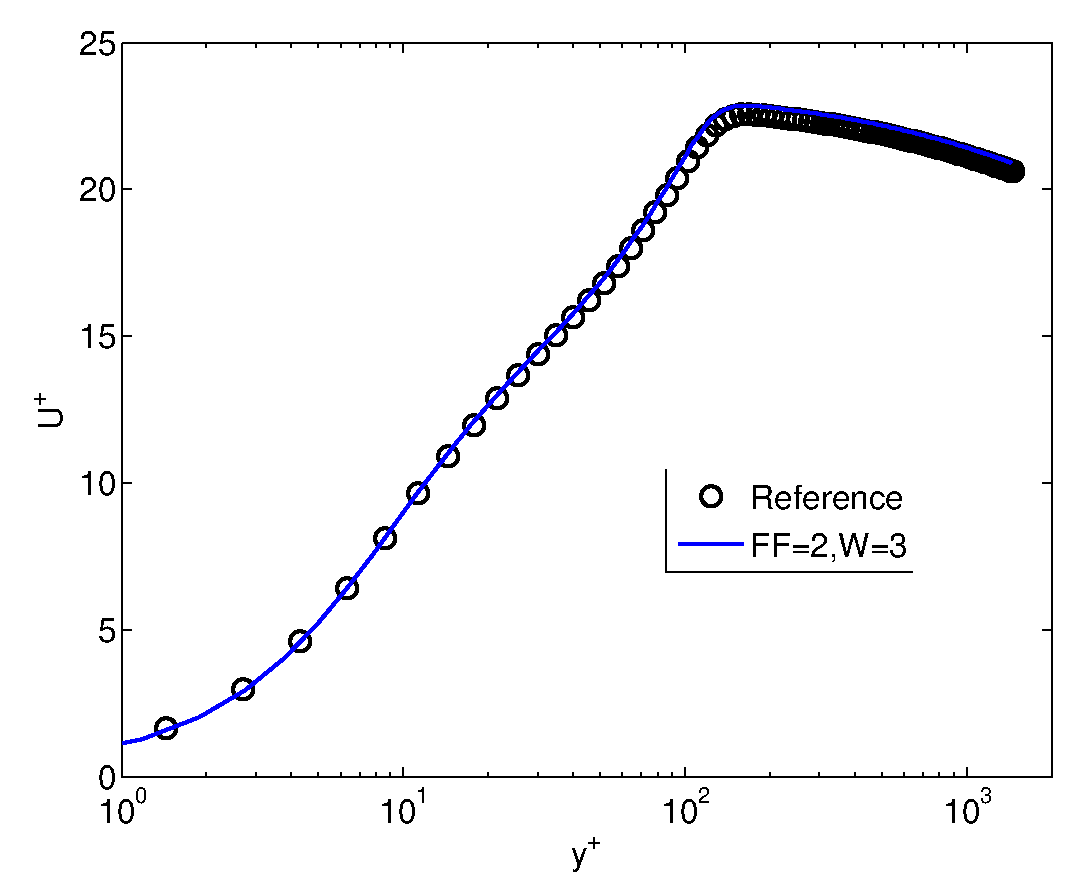
\includegraphics[width=0.9\columnwidth]{outflow_ff2w3_meanup}
		\caption{Mean flow}
		\label{fig:outflow_ff2w3_up}
	\end{subfigure}
	\begin{subfigure}[h]{0.45\textwidth}
		\centering
		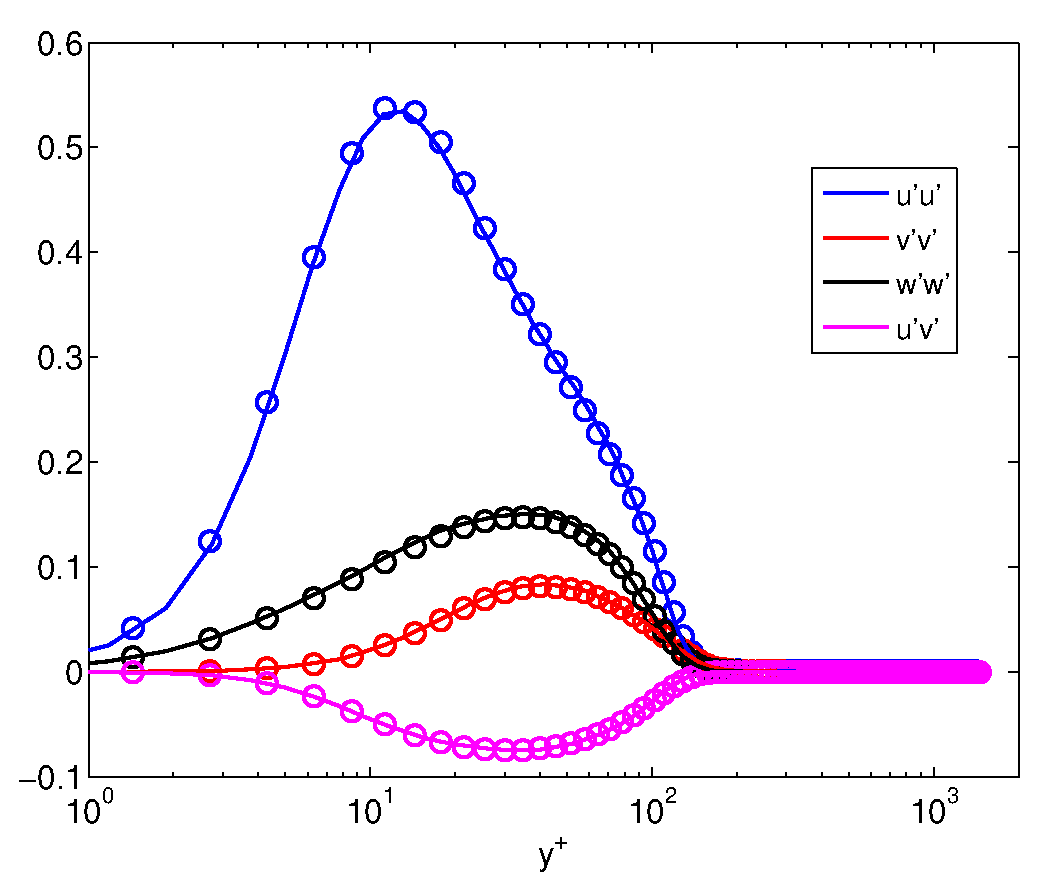
\includegraphics[width=0.9\columnwidth]{outflow_ff2w3_rs}
		\caption{Reynolds stresses}
		\label{fig:outflow_ff2w3_rs}
	\end{subfigure}
	\caption{Comparison of mean streamwise velocity and Reynolds stresses for a truncated domain with the far-field being 2 chords away and the outflow 4 chords away from the leading edge.}
	\label{fig:outflow_ff2w3_u_rs}
\end{figure}
\begin{figure}
	\centering
	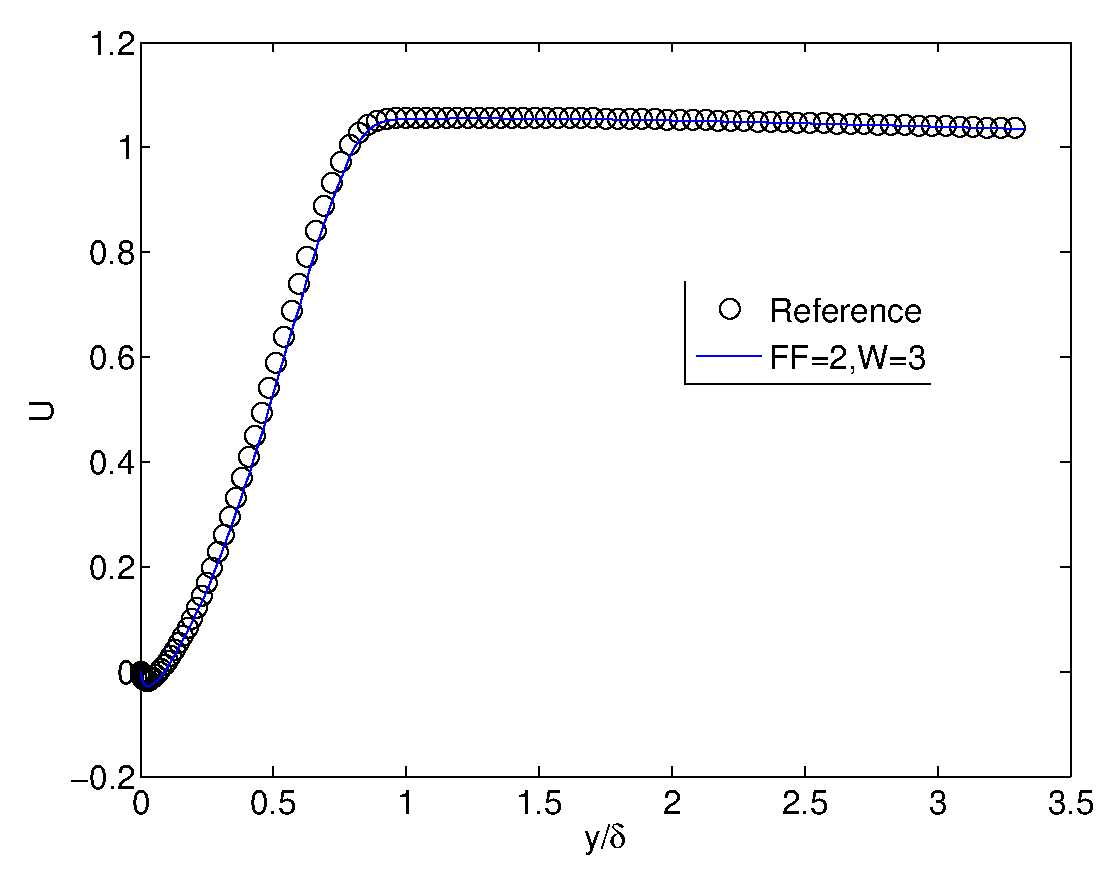
\includegraphics[width=0.5\columnwidth]{outflow_ff2w3_meanu_085}
	\caption{Comparison of mean streamwise velocity profile in the separated region on the suction-side ($x/c=0.85$).}
	\label{fig:outflow_ff2w3_meanu_sep}
\end{figure}
Figure~\ref{fig:domain_ff2w3} shows a 2D x-y section of the truncated domain with figure~\ref{fig:grid_ff2w3} showing a close-up of the grid near the leading edge. The setup is very similar to the reference case (figure~\ref{fig:domain_grid_reference}). Figure~\ref{fig:la2_ff2w3} shows the isocontours of flow structures identified by the $\lambda_{2}$ criterion, which look qualitatively similar to the ones seen in the reference case (figure~\ref{fig:la2_reference}).
\begin{figure}[h]
	\centering
	\begin{subfigure}[b]{0.45\textwidth}
		\centering
		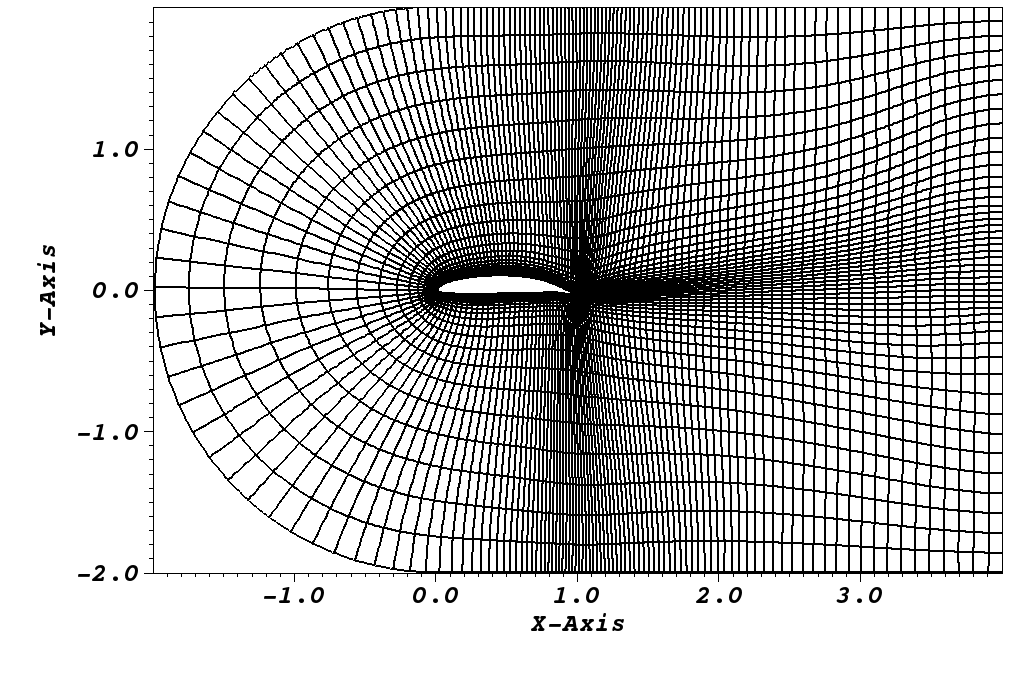
\includegraphics[width=1.0\columnwidth]{domain_ff2w3}
		\caption{Simulation domain}
		\label{fig:domain_ff2w3}
	\end{subfigure}
	\begin{subfigure}[b]{0.45\textwidth}
		\centering
		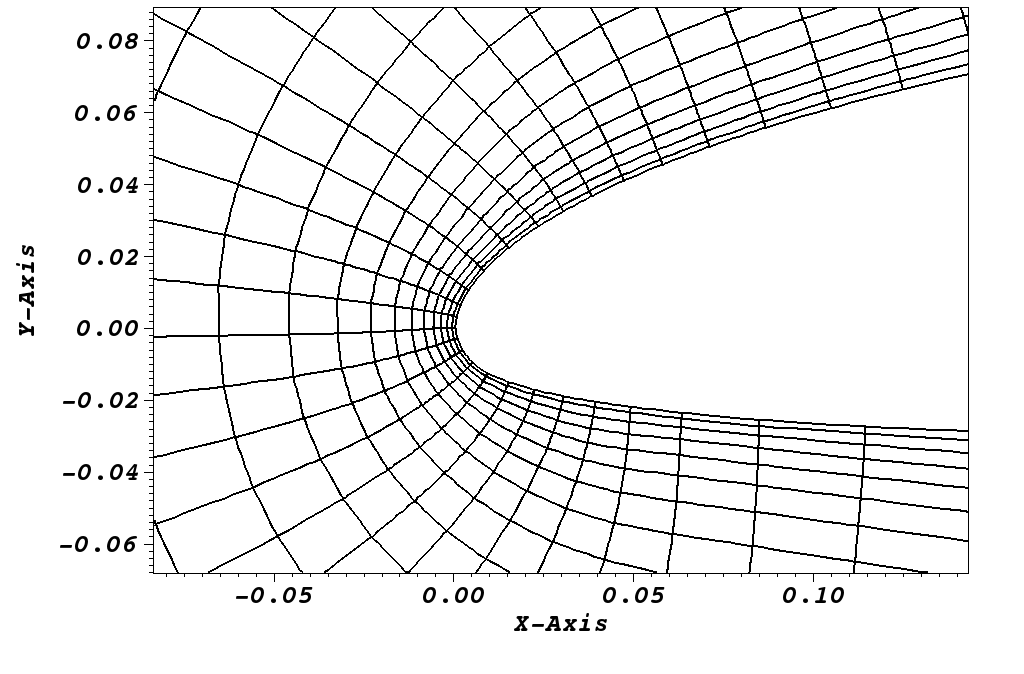
\includegraphics[width=1.0\columnwidth]{grid_ff2w3}
		\caption{Spectral-element grid}
		\label{fig:grid_ff2w3}
	\end{subfigure}
	\caption{Truncated simulation domain (a) and a close-up (b) near the leading edge, of the orthogonal and structured spectral-element grid. Domain is truncated such that the far-field is 2 chords from the airfoil and the outflow is 3 chords downstream from the trailing edge.}
	\label{fig:domain_grid_ff2w3}
\end{figure}

\begin{figure}
	\centering
	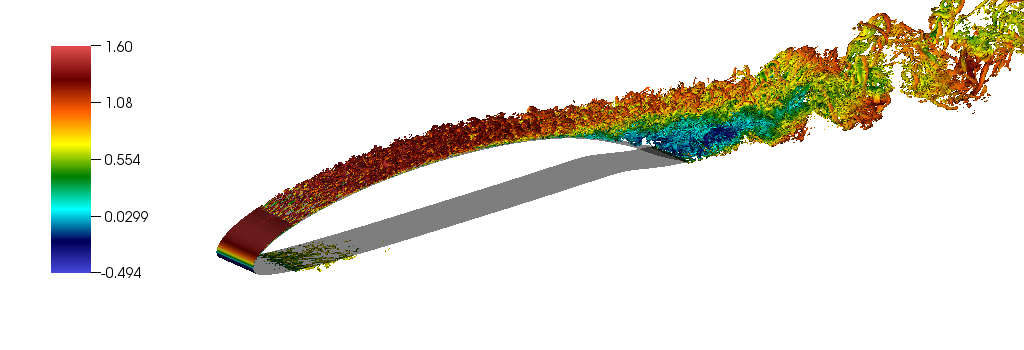
\includegraphics[width=0.9\textwidth,height=0.35\textwidth]{la2_ff2w3.png}
	\caption{Visualization of the instantaneous flow structures in the truncated domain. The flow structures are identified by the isocontours of the $\lambda_{2}$ criterion and are colored by streamwise velocity.}
	\label{fig:la2_ff2w3}
\end{figure}

%\FloatBarrier
\section{Conclusion}

A comparison of the energy-stabilized outflow boundary condition \citep{dong2014} with the standard stress-free boundary condition is performed when the outflow boundary is 4 chords downstream of the trailing edge. The energy-stabilized outflow is seen to have negligible effect on the boundary layer developing on the wing surface. Test cases with different truncated domains show that in a C-grid type mesh topology, flow distortion effects due to the boundary conditions are minimized when the far-field boundary is 2 chords away from the airfoil and the outflow boundary is 3 chords downstream from the trailing edge. The result however is subject to the imposition of a RANS velocity field as Dirichlet boundary condition on the far-field boundaries and the energy-stabilized outflow boundary condition on the outflow boundaries of the LES simulation.
%===============================================================================

%\FloatBarrier
%\begin{footnotesize}
%\bibliography{scigenbibfile.Donald+Duck.Mickey+Mouse.Goofy+G.+Goof}\bibliographystyle{acm}
%\end{footnotesize}
%
%\end{document}



%------------------------------------------------------------------------------
% Bibliography
%------------------------------------------------------------------------------
%
%\clearpage
\bibliographystyle{jfm}
\bibliography{licentiate}
%
\IfFileExists{validation/validation.bbl}{\input{validation/validation.bbl}}{}


%===============================================================================
%                            END PAPER
%===============================================================================
\end{paper}
}{}


%===============================================================================
%                            END PAPER
%===============================================================================
\end{paper}
